
%
%
%
%
%

\chapter{Results}
\section{3D Dataset, EM Mitochondria Labelling}
To demonstrate the image segmentation pipeline in all its parts we choose to use a EM Mitochondria dataset because it is a natural dataset with objects which are not easily distinguishable, and still has good labeled data. The single training image of size $1024 \times 768 \times 165$ was split into 82 by 82 by 82 cubes and super-pixels where constructed with $S=10$ and $M=9$ producing a graph with 921 nodes on average. We then trained the Naive Max classifier on a unary model, Mean Field and LoopyBP on a pairwise model and LoopyBP on two data dependent pairwise models. The results show a clear superiority of pairwise models over unary models. Amongst the pairwise models it can be benificial to use a more complex data dependent model but the score variance is too high for a statistically significant difference. Surprisingly we found that with a $\lambda =100$ Mean Field performed close to LoopyBP with lower training time. See Figure \ref{fig:mitochonCmpMethods} for details. 


\begin{figure}[H]
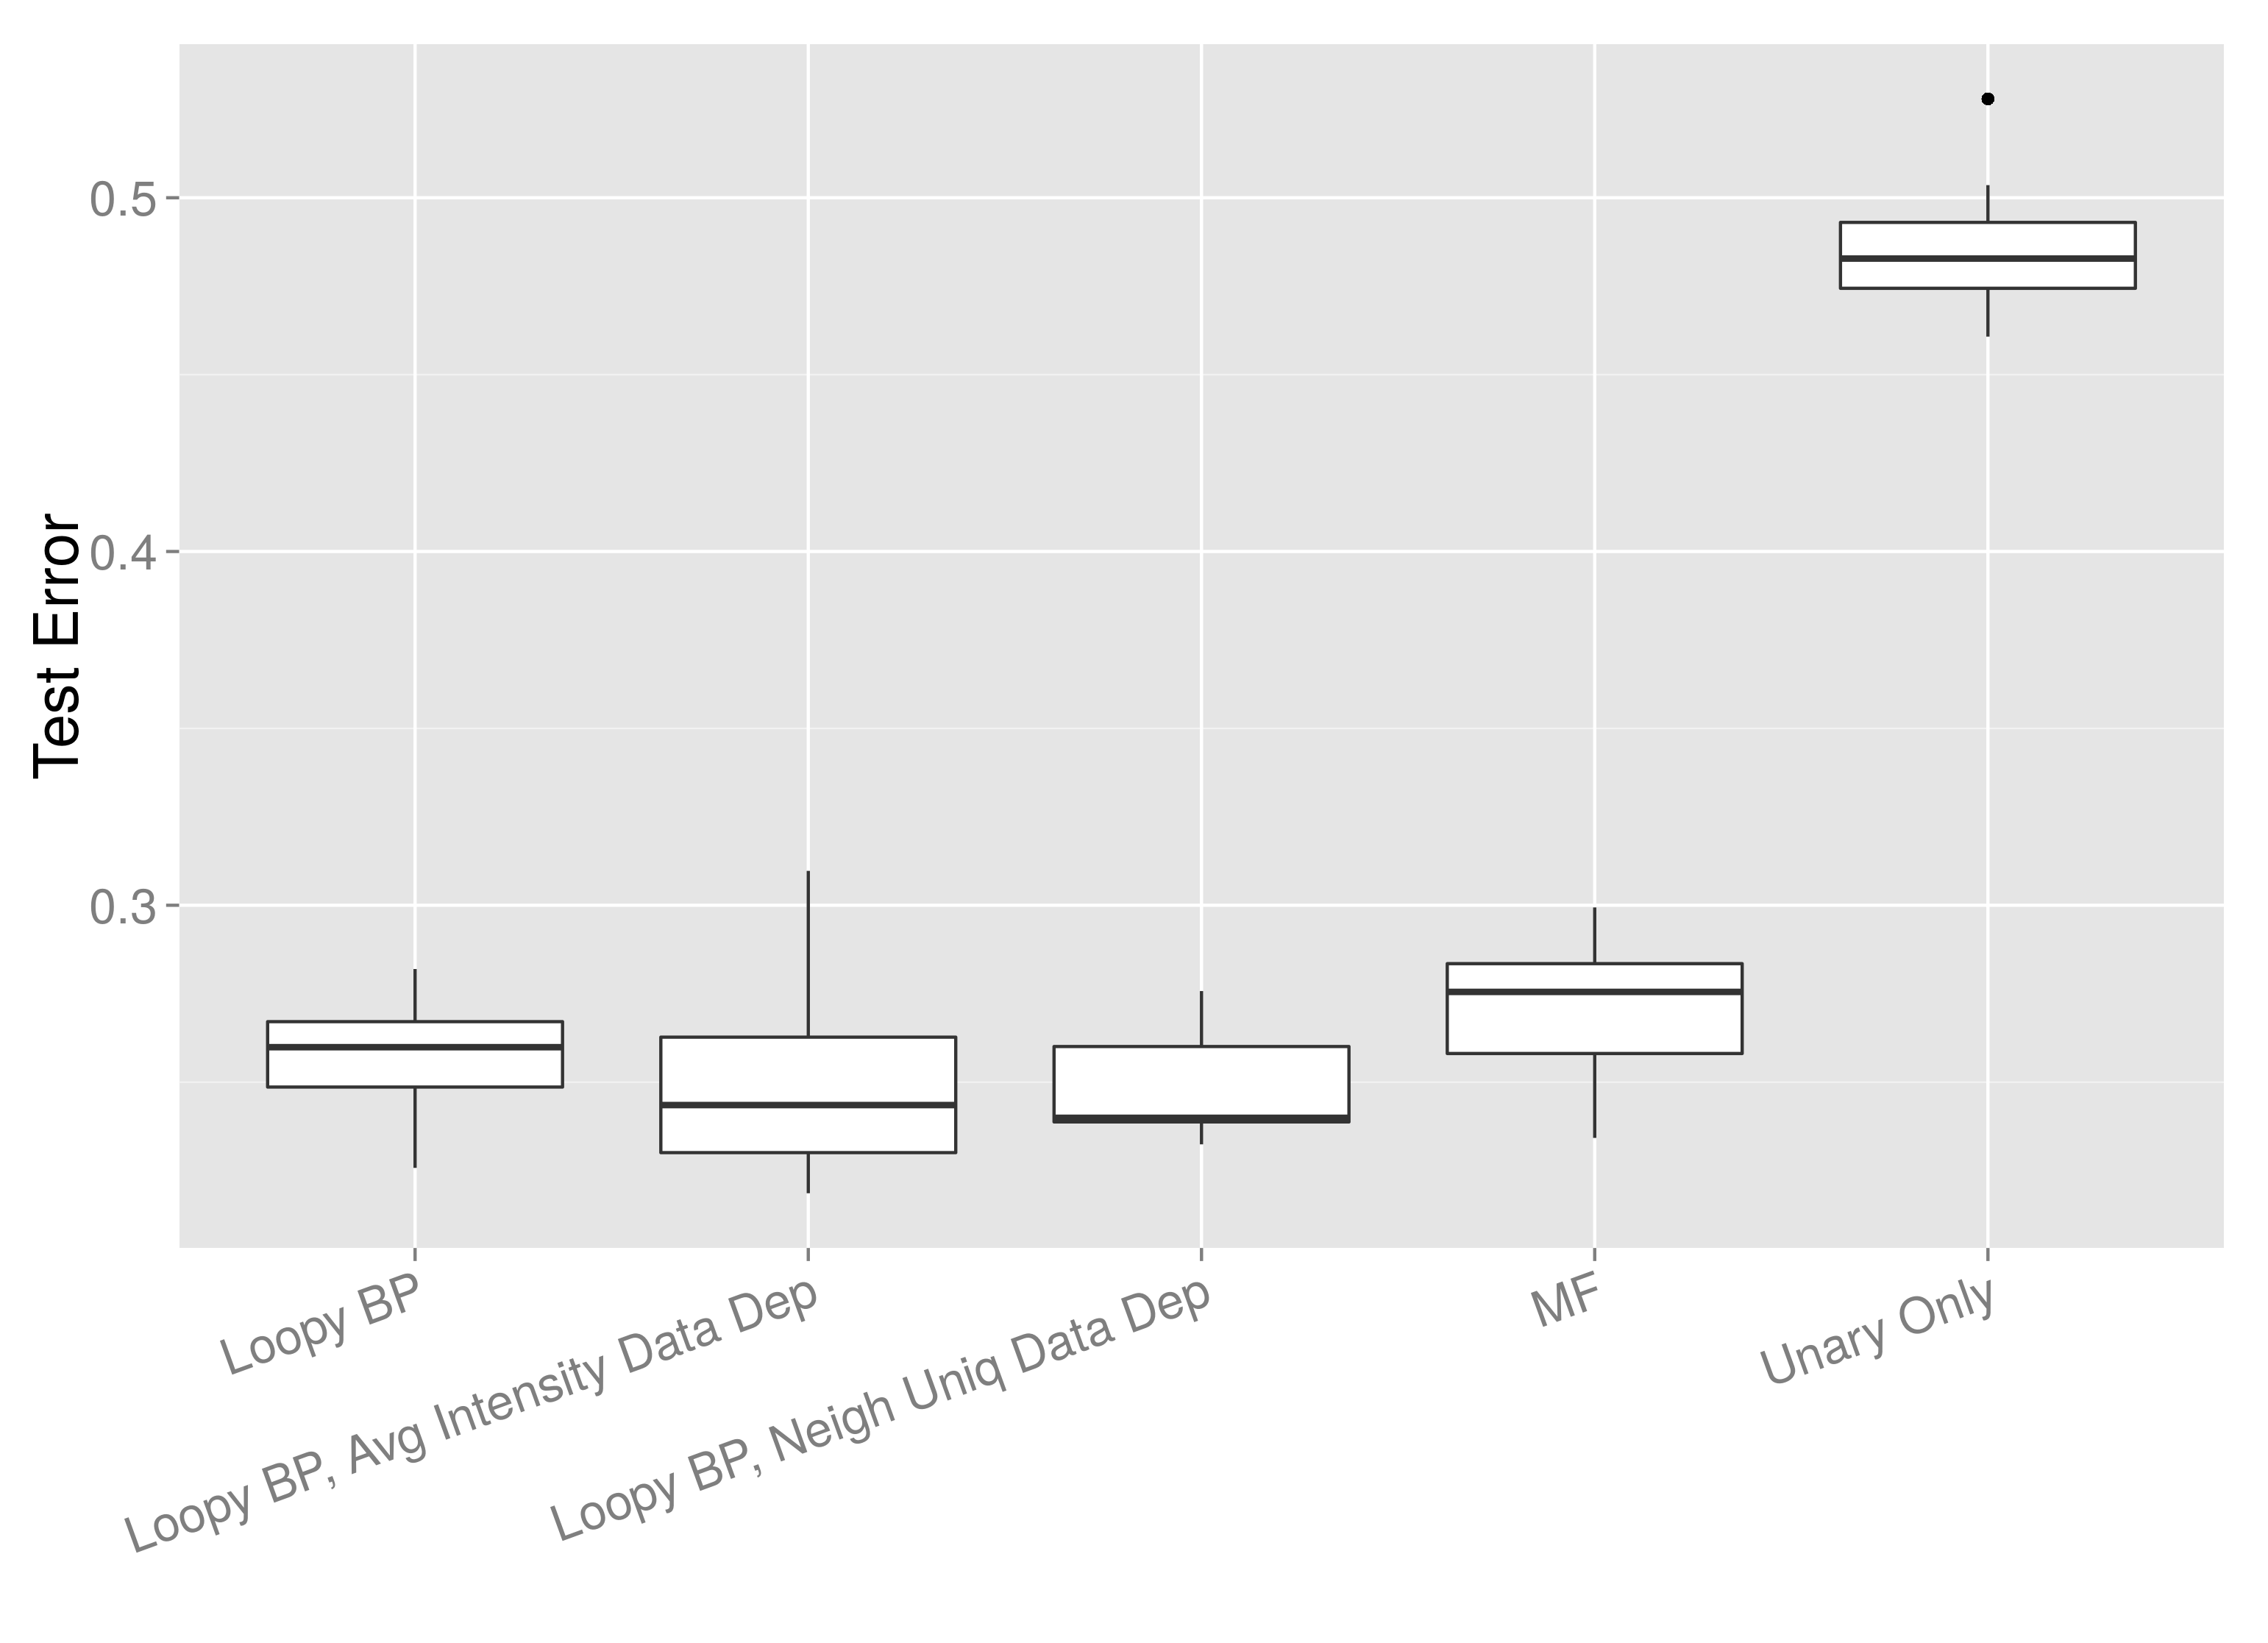
\includegraphics[width=0.8\textwidth]{images/mitochonSplit_testError_end.png}
  \caption {  Over 30 rounds we trained the SSVM with different using different models and different max oracle functions. LoopyBP and MF where trained on a simple pairwise model as in \ref{sec:pariwiseSimple}. Naive Max oracle was trained a Unary only model see \ref{sec:unaryModel}. Additionally we trained two data dependent pariwise models (see section \ref{sec:dataDep}) with LoopyBP max-oracle. The data dependent pairwise transition binning function "Avg Intensity" groups neighbouring nodes by the difference in the mean intensity inside each super-pixel, the function "Neigh Uniq" calcluates how many standard deviations away the mean of node A is from the distribution of intensities in the one hope neighbourhood of node B. Data:( EM Mitochondira Labeled Image split into $82^3$ cubes with super-pixels of size $S=10$ \cite{mitochondriaData} ) } 
  \label{fig:mitochonCmpMethods}
\end{figure}


\section{Sparse Transition Probability Tables}
During our exploration of different datasets we saw high variance on whether the pairwise models increases accuracy as compared to the baseline naive unary max oracle. To examin which situations the pairwise term is particularly helpful we designed as set of synthetic experiments. For details on the data generation functions see Appendix \ref{sec:synthDataGen}. In the following experiments we generated data with a significant amount of noise and set rules for how many labels are allowed to be adjacent to any label A for all other labels. We call the probability that two labels are allowed to be neighbours \inputArgs{dataGenNeighProb}. If we were to allow any label to be next to any other label then the only thing the pairwise term can learn is that super pixels generally occure in groups. So they are generally more likely to occur next to one of their own label versus any other. But by restricting only few labels to be allowed as neighbours we give the pairwise term a target which contains many zeros and hence will have a greater impact on the decoding energy. In the following graph we show the accuracies of pairwise versus unary model while changing the probability that any 2 classes are allowed to be neighbours.

\begin{figure}[H]
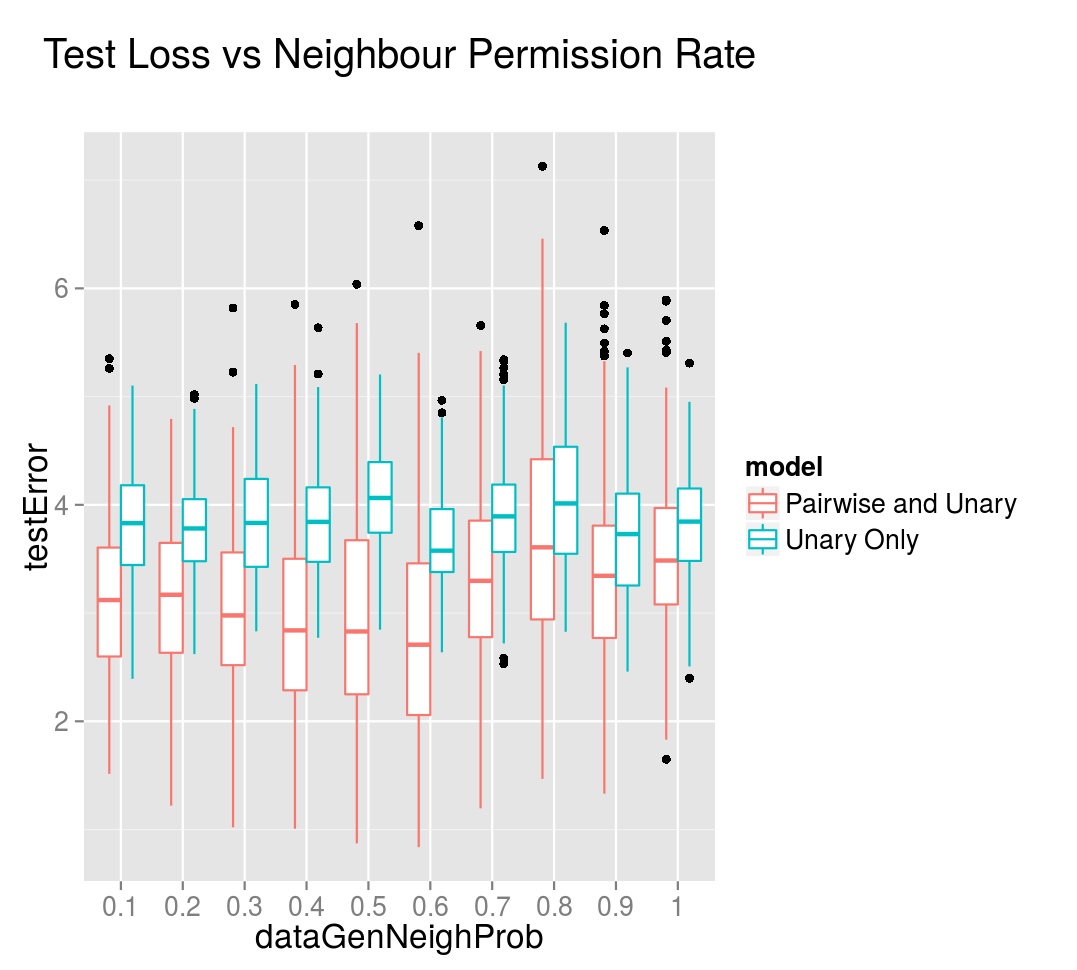
\includegraphics[width=1\textwidth]{images/tesLoss_vs_Neighbour_permission.png}
  \caption { As the \inputArgs{datagenNeighProb} decreases it creates a more sparse transition probability matrix which makes it easier for the pairwise models to identify this information. Once below 0.3 the pairwise benefit starts decreasing again because the likelihood of the most of the image being the background label increases. Data ( SynthData, WhiteNoise:0.40 SquarImgSize:30 OsilNoise:0.40 SupSqrColorShift:0.0 SuperPix, S:5, M:5, Max Decoding:LoopyBP ) } 
  \label{fig:neighprobVSloss}
\end{figure}

As the reader can see the largest difference between unary and pairwise occurs in the middle of the graph. This is because as \inputArgs{dataGenNeighProb} goes to 1.0 all classes can be adjacent to all others. As it approaches 0.0 the image becomes mostly background because that label is reserved as a fallback when all other labels are not allowed due to the neighbouring rules. In Table \ref{table:neigh1} the reader can inspect columns of the transition probability and the weights learned in the pariwise model for data using this transition probability table. Notice, those label pairs which have the highest transition probability also have the highest weight in the corresponding learned pairwise potential column. In contrast table \ref{table:neigh2} does not have this correspondence. BCFW does not have an objective of learning the correct transition probabilities but rather to decrease the hinge loss. For this objective it only alters the direction of $\weightVect$ if that portion of the feature vector is usefull in destingushing data. Hence when the transition probability is not sufficiently distinguishable between images it will not be learned. 
\begin{table}
\caption{Transitions tables using \inputArgs{dataGenNeighProb=0.4} }
\label{table:neigh1}
\subcaption*{True Transition probability between labels}
\centering
\begin{tabular}{ c c c c}
	0.000e+00 &	4.245e-01 & 3.271e-02 &	0.000e+00 \\
	4.245e-01 &	0.000e+00 &	2.861e-02 &	0.000e+00 \\
	3.271e-02 &	2.861e-02 &	1.667e-03 &	1.333e-02 \\
	0.000e+00 &	0.000e+00 &	1.333e-02 &	0.000e+00 \\
\end{tabular}
\bigskip
\subcaption*{Learned Pairwise Weights}
\begin{tabular}{ c c c c}
  -7.349e-04 & 4.557e-04 & 3.112e-04 & -2.030e-05 \\
  4.557e-04 & -1.305e-04 & -3.408e-04 & -1.313e-04 \\
  3.112e-04 & -3.408e-04 & -1.149e-04 & 1.250e-04 \\
  -2.030e-05 & -1.313e-04 & 1.250e-04 & -5.570e-05 \\
\end{tabular}
\end{table}
\begin{table}
\caption{ Transition tables using \inputArgs{dataGenNeighProb=1.0}: }
\label{table:neigh2}
\subcaption*{True Transition probability between labels}
\centering
\begin{tabular}{ c c c c}
  1.046e-01 & 1.106e-01 & 1.120e-01 & 2.292e-03 \\
  1.106e-01 & 1.061e-01 & 1.099e-01 & 2.500e-03 \\
  1.120e-01 & 1.099e-01 & 1.092e-01 & 2.778e-03 \\
  2.292e-03 & 2.500e-03 & 2.778e-03 & 1.389e-04 \\
\end{tabular}
\bigskip
\subcaption*{Learned Pairwise Weights} 
\begin{tabular}{ c c c c}
  7.650e-05 & 3.878e-04 & 2.306e-04 & 4.022e-05 \\
  3.878e-04 & 2.015e-04 & 3.430e-04 & 4.590e-05 \\
  2.306e-04 & 3.430e-04 & -7.471e-05 & 3.638e-05 \\
  4.022e-05 & 4.590e-05 & 3.638e-05 & -4.405e-05 \\
\end{tabular}

\end{table} 
With the sparse transition probability explanation for the pairwise advantage in mind we can construct a dataset which should give more advantage to the pariwise model by making the super-pixels exactly equal to the supersquares. This configuration should result in transition probabilities from the label to itself (the diagonal) being as sparse as the rest of the matrix. In Figure \ref{fig:s_equals_superSquare} we see the expected result, that the distance between the pairwise and unary model increases as we farther increase the sparsity of the transition probability matrix. 


\begin{figure}
\centering
\caption{Test Error vs Label Transition Sparsity}
\subcaption*{With Superpixel size == SuperSquare size}
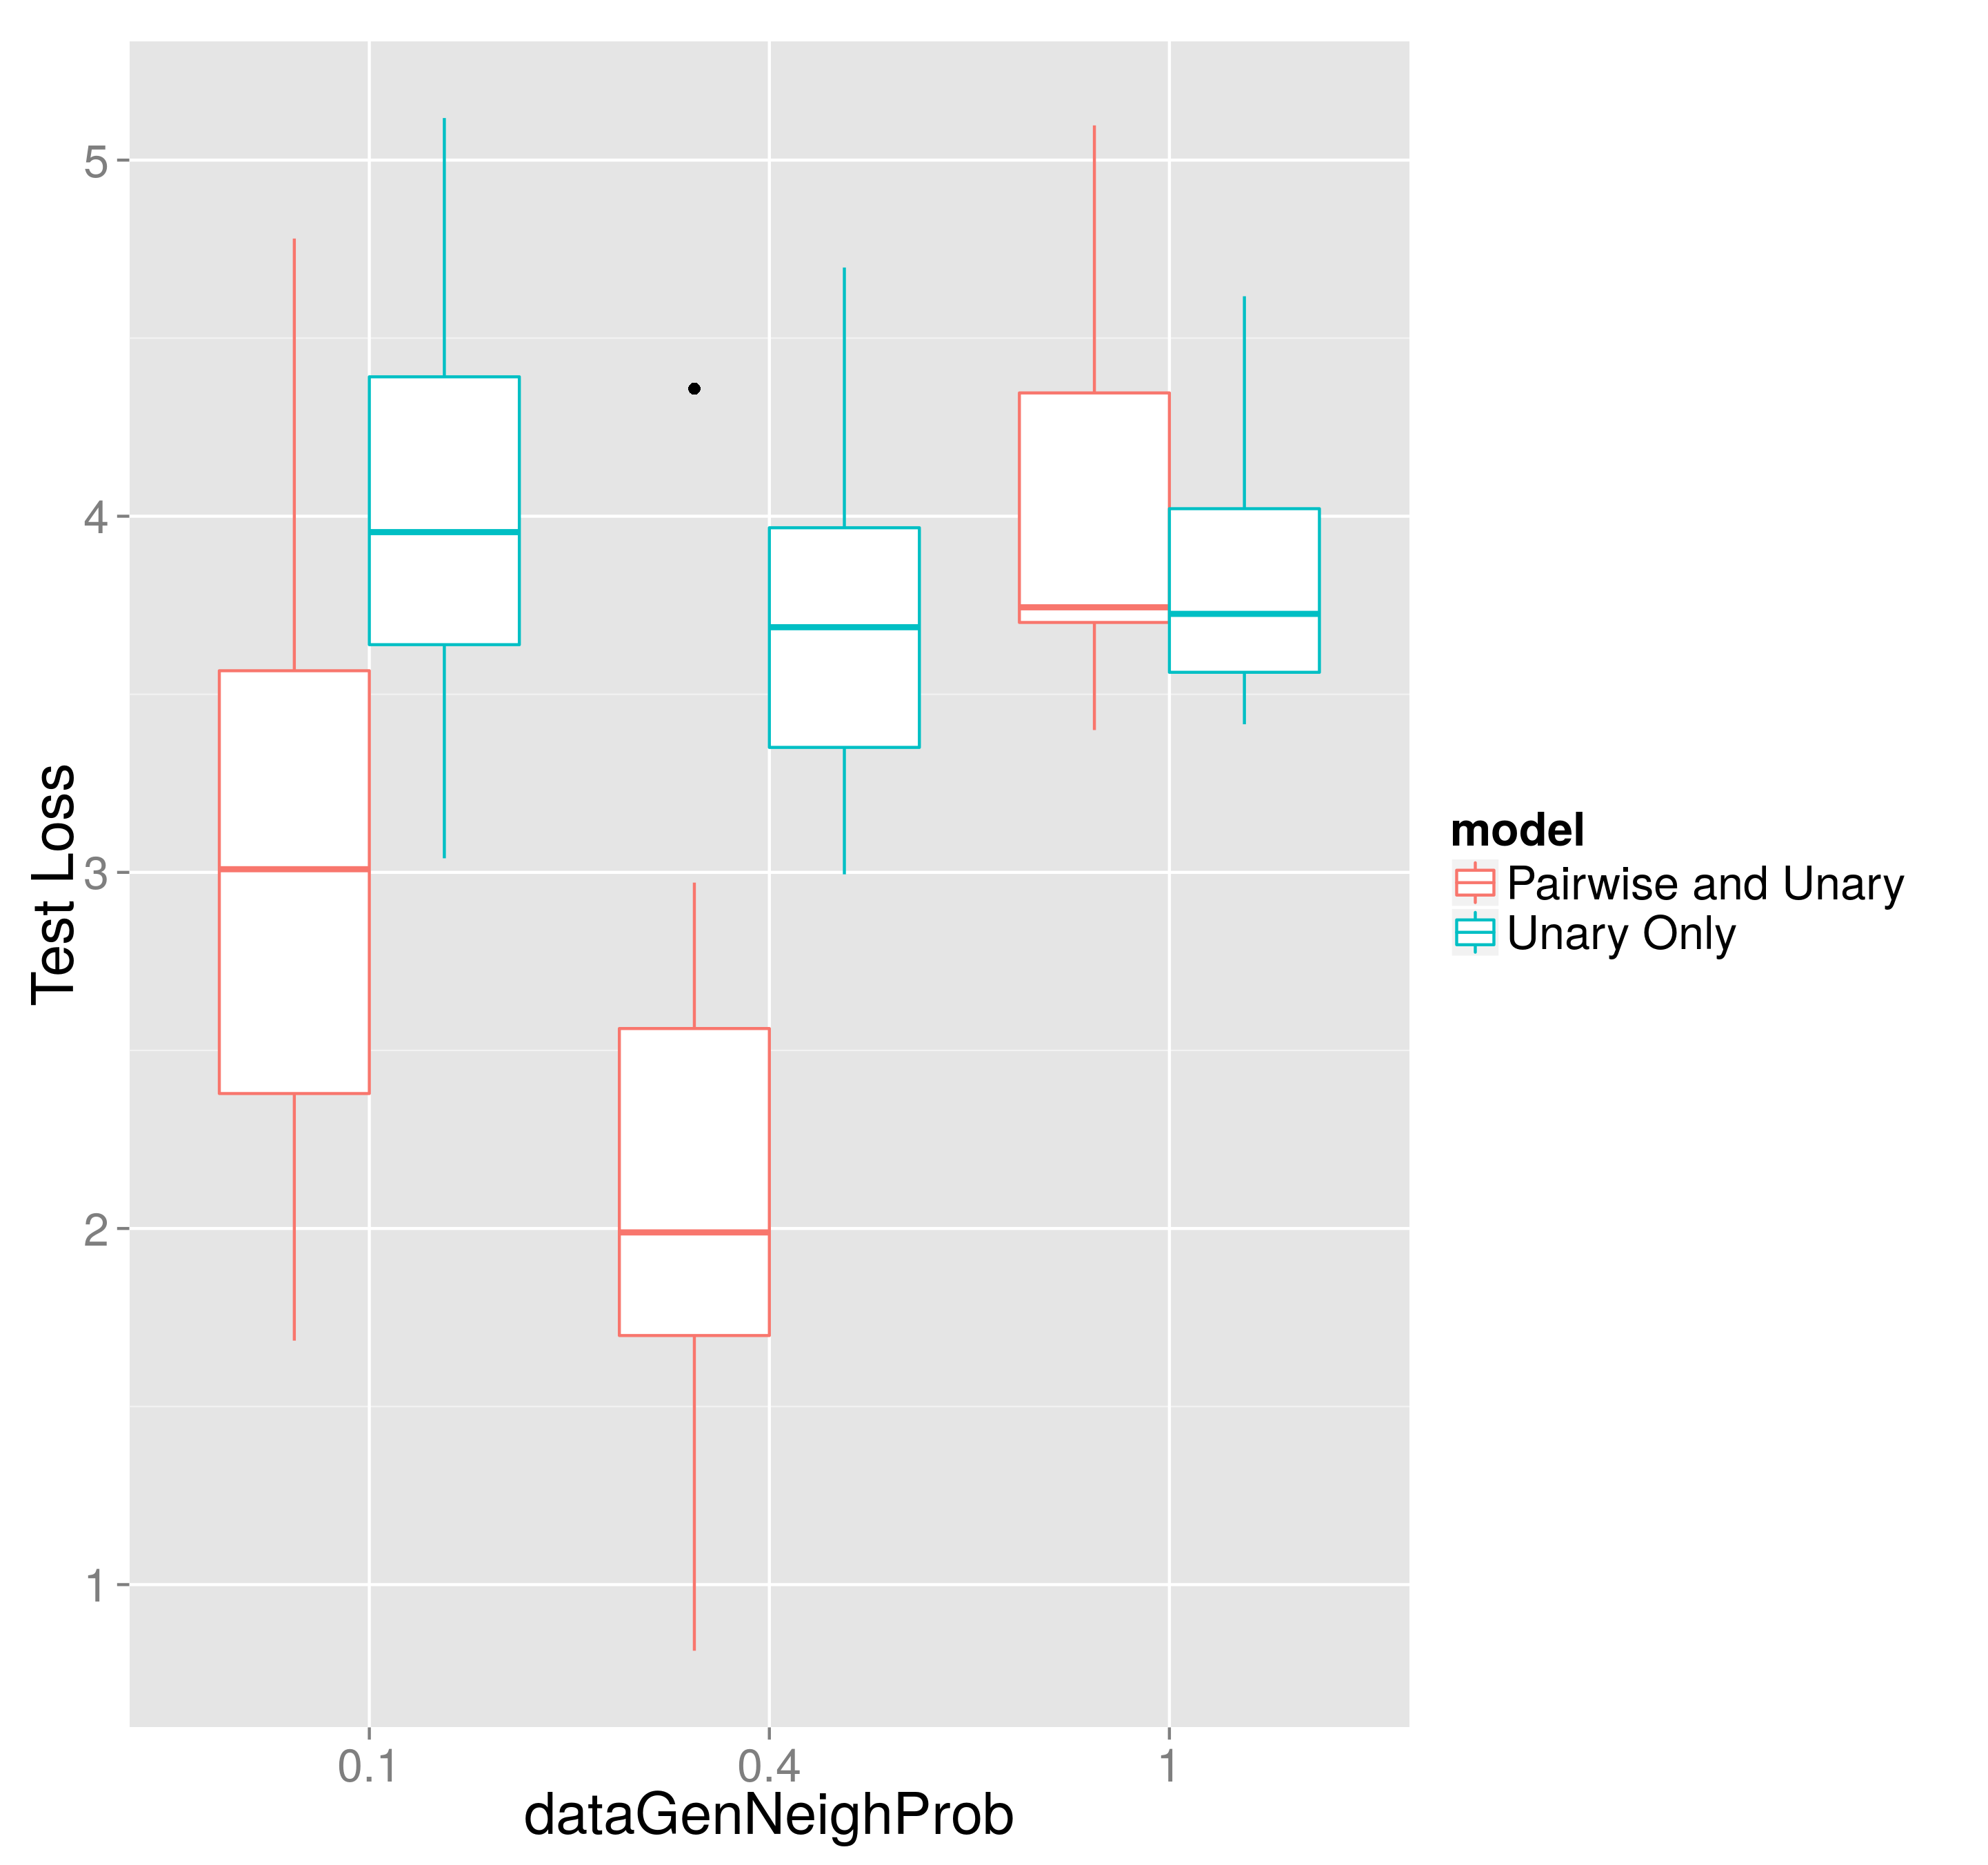
\includegraphics[width=1.0\textwidth]{images/neighProb_s_equals_supSquare.png}
\caption{ The figure shows a substantial improvement in the test Error for the pairwise model. These results can be compared to \ref{fig:neighprobVSloss} which is the same experiment but with smaller super pixels. Since in this experiment we set the superpixels equal to the supersquare size the diagonal of the transition probability matrix is just as sparse as the rest.  Data ( SynthData, WhiteNoise:0.40 SquarImgSize:30 OsilNoise:0.40 SupSqrColorShift:0.0 SuperPix, S:30, M:30, Max Decoding:LoopyBP ) }
\label{fig:s_equals_superSquare}
\end{figure}


\section{Prediction Smoothing}\label{smoothness}
By visual inspection of label predictions we subjectively observed a trend of the pairwise models performing better when disconnected single lables in clusters of others labels is unlikely. 
In figure \ref{fig:smooth1} we can see the upper row of predicted labels by the pairwise model is much smoother than the lower row of unary model predictions.  As described above the supersquares are always of equal size and in this configuration contain several superpixels internally. The image is not perfeclty smoothed into squares because we jointly optimize pairwise and unary factors. 
Figure \ref{fig:smoothNuclie} gives evidence for the same understanding of smoothness as figure \ref{fig:smooth1} but with real world data. Again we see that the pairwise model has less standalone super pixel labels indicating that the pairwise term is working as expected. But in this particular experiment the the pairwise term also had a negative effect as on the lower side of the nuclei cluster is another set of high contrast objects which are only slightly disconnected from the main body. These nearby easily mistaken objects are all grouped into the main nuclei cluster in using the pairwise term resukt in a worse score than the few misslabeling made by the unary model. Hence we must be mindful of the way in which we are including the spacial relations into our model, as in this datasets where one must consider that there may be a separation between groups of classes which is less than one super pixel wide. One way to combat this could be to set the compactness parameter for the SLIC preprocessing very low so that thin long superpixels could be placed between the two groups of classes. 
\begin{figure}[H]
  \centering
  
  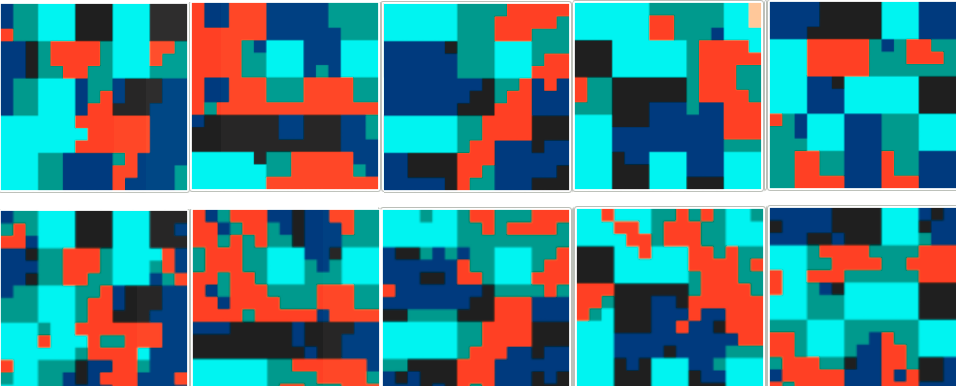
\includegraphics[width=0.8\textwidth]{images/compare_smoothness_syntheticData_pariwise_v_unary.png}
  \caption{ This figure shows the predicted labels per pixel for a pairwise model in the top row and a unary only model in the bottom row. By visual inspection the reader can see that the top pairwise model is more smooth in that the blobs of labels are more connected and generally in larger collections. While the bottom unary model output frequently has a single super pixel with a label surrounded by larger groups of distinct labels. Data ( SynthData, WhiteNoise:0.40 SquarImgSize:30 OsilNoise:0.40 SupSqrColorShift:0.0 SuperPix, S:30, M:30, Max Decoding:LoopyBP/NiveMax )} 
  \label{fig:smooth1}
\end{figure} 
\begin{figure}
\begin{subfigure}{.5\textwidth}
  \centering
  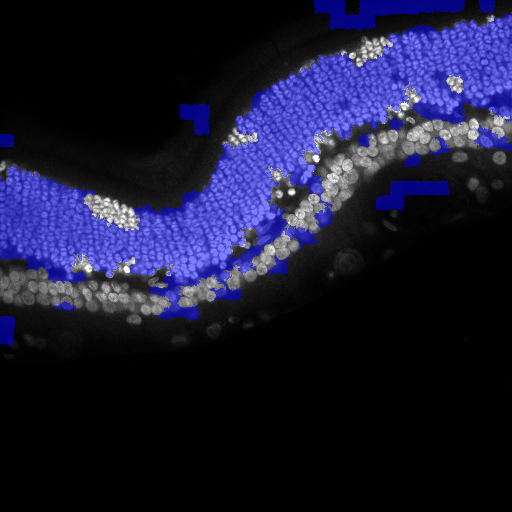
\includegraphics[width=0.9\linewidth]{images/3dnone_0-train_predict_unary.png}
  \caption{Unary Model prediction}
  \label{fig:smoothNuclieUnary}
\end{subfigure}%
\begin{subfigure}{.5\textwidth}
  \centering
  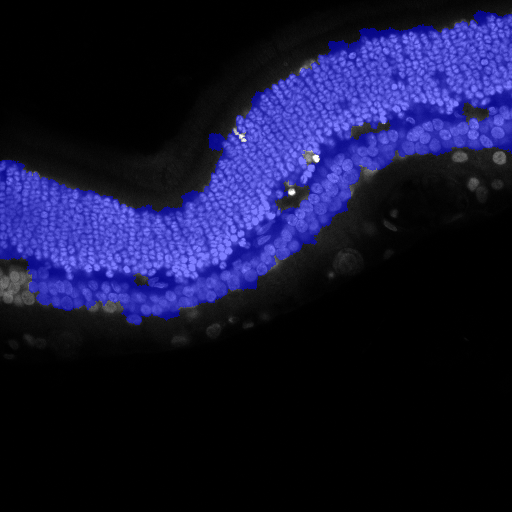
\includegraphics[width=0.9\linewidth]{images/3dnone_0-train_predict_pairwise.png}
  \caption{Pairwise Model prediction}
  \label{fig:smoothNucliePair}
\end{subfigure}
\caption{ Per-superpixel predicted labels are superimposed on the raw image. This Nuclei detection dataset only has foreground and background hence we only colored the Nuclei label foreground predictions. The reader can observe that the Unary model (a) has more disconnected components than the Pairwise model (b). In this particular dataset the nuclei are always connected in one large object hence giving pairwise model an advantage to not make this kind of error. Data( Single Channel 3D Nuclei \cite{ucsbData}) }
\label{fig:smoothNuclie}
\end{figure}
\section{Impact of the Regularizer }\label{sec:Lambda}
Out of all the tuning parameters \inputArgs{lambda} needs to be adjusted most carefully, as it determines the freedom $W$ has. In the optimization function $\lambda$ can be interpreted as weighing the size of the margin and the actual loss defined in the slack variable (see equation \vref{optimizationFunc}). As we can see in figure \ref{fig:lambda1} choosing the right lambda for your problem is crucial for the final outcome. This pattern in test error can be further explained when looking at the structured hinge loss over rounds, Figure \ref{fig:lambda2}. We can see that for low lambdas the Structured Hinge loss $\shloss$ does not decrease over meaning that the lambda was so restrictive on the norm of $\weightVect$ that BCFW could not find a piece of information which was usefull enough to warrent changing the norm of $\weightVect$. 

\begin{figure}
  \centering
    \figuretitle{ Test Error vs Lambda, Using Untransformed Features}
  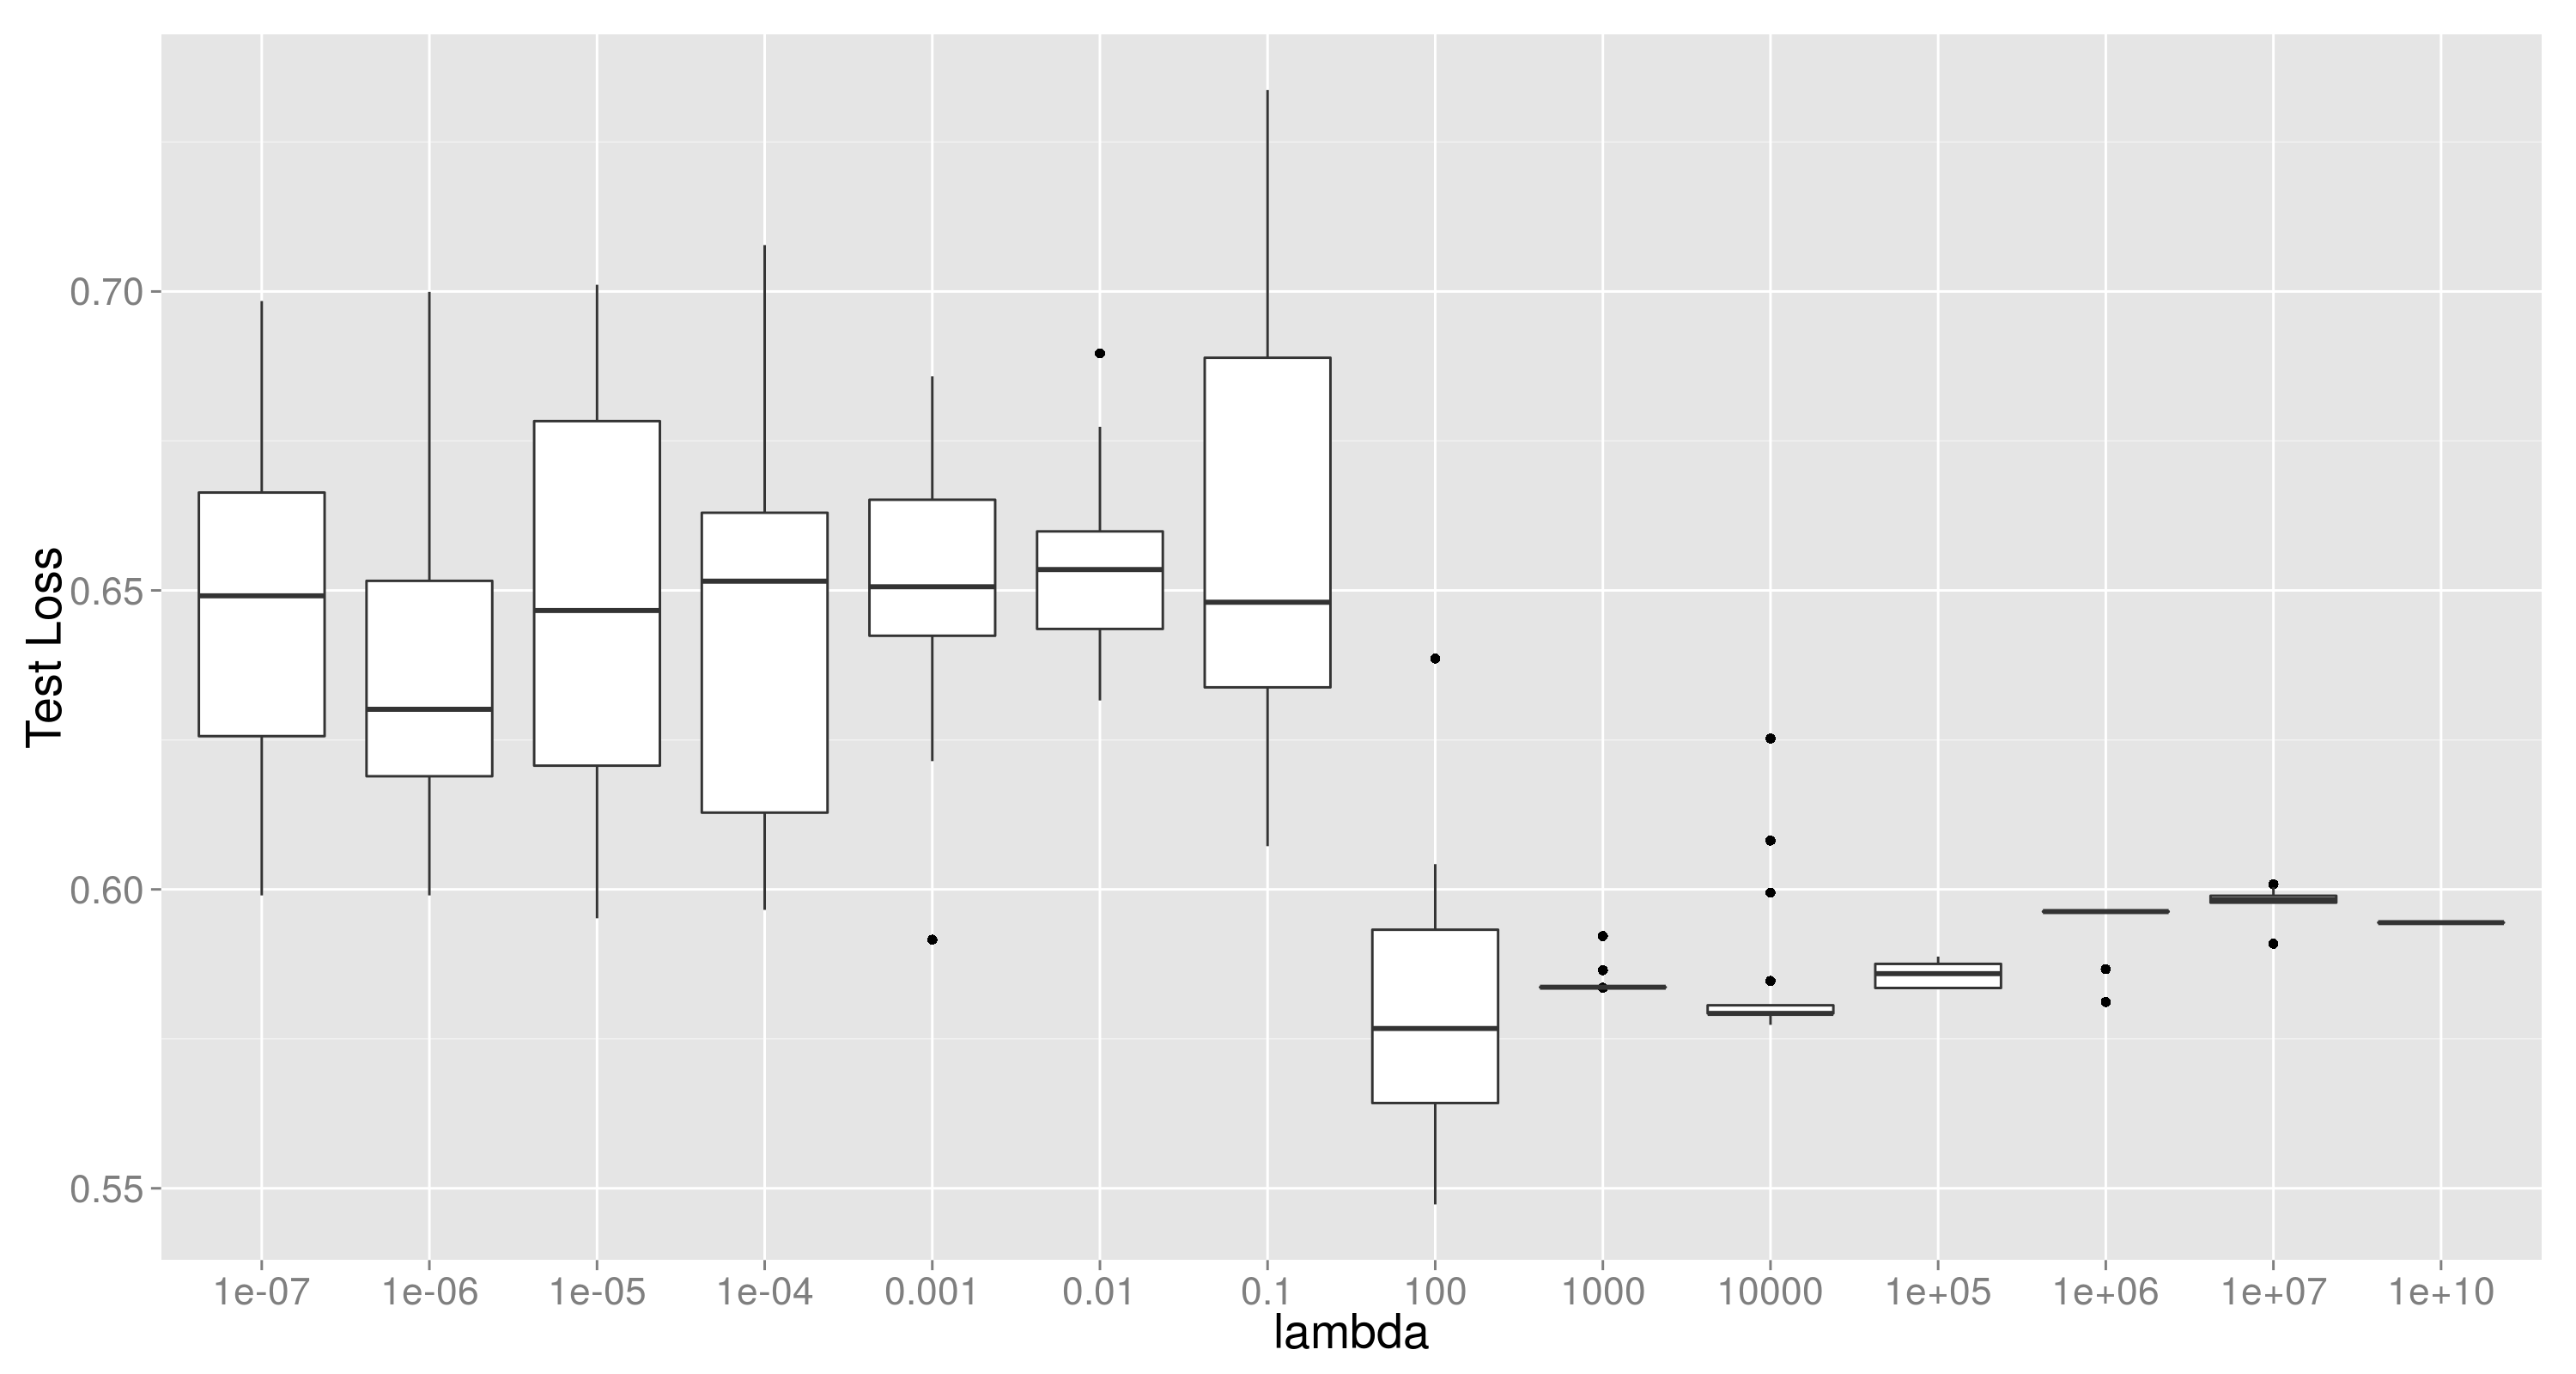
\includegraphics[width=1.0\textwidth]{images/tesatError_vs_lamda_msrc.png}
  \caption{   Displayed are the test scores of the same model run with different regularization lambdas. The distribution displayed was produced by insample cross validation. We can see a clear separation between lambdas which are not strict enough to result in good convergence ($\geq 100, \leq 10000$) and those which do not converge ($\leq 0.1$). Additionally lambdas which are too strict result in lower accuracy again do to them not allowing full exploration of the relations between the features ($\geq 100000$). Data( MSRC version 2 \cite{msrcDataSet}) } 
  \label{fig:lambda1}
\end{figure} 

\begin{figure}
  \centering
  \figuretitle{Structured Hinge Loss over time, faceting on different lambdas}
  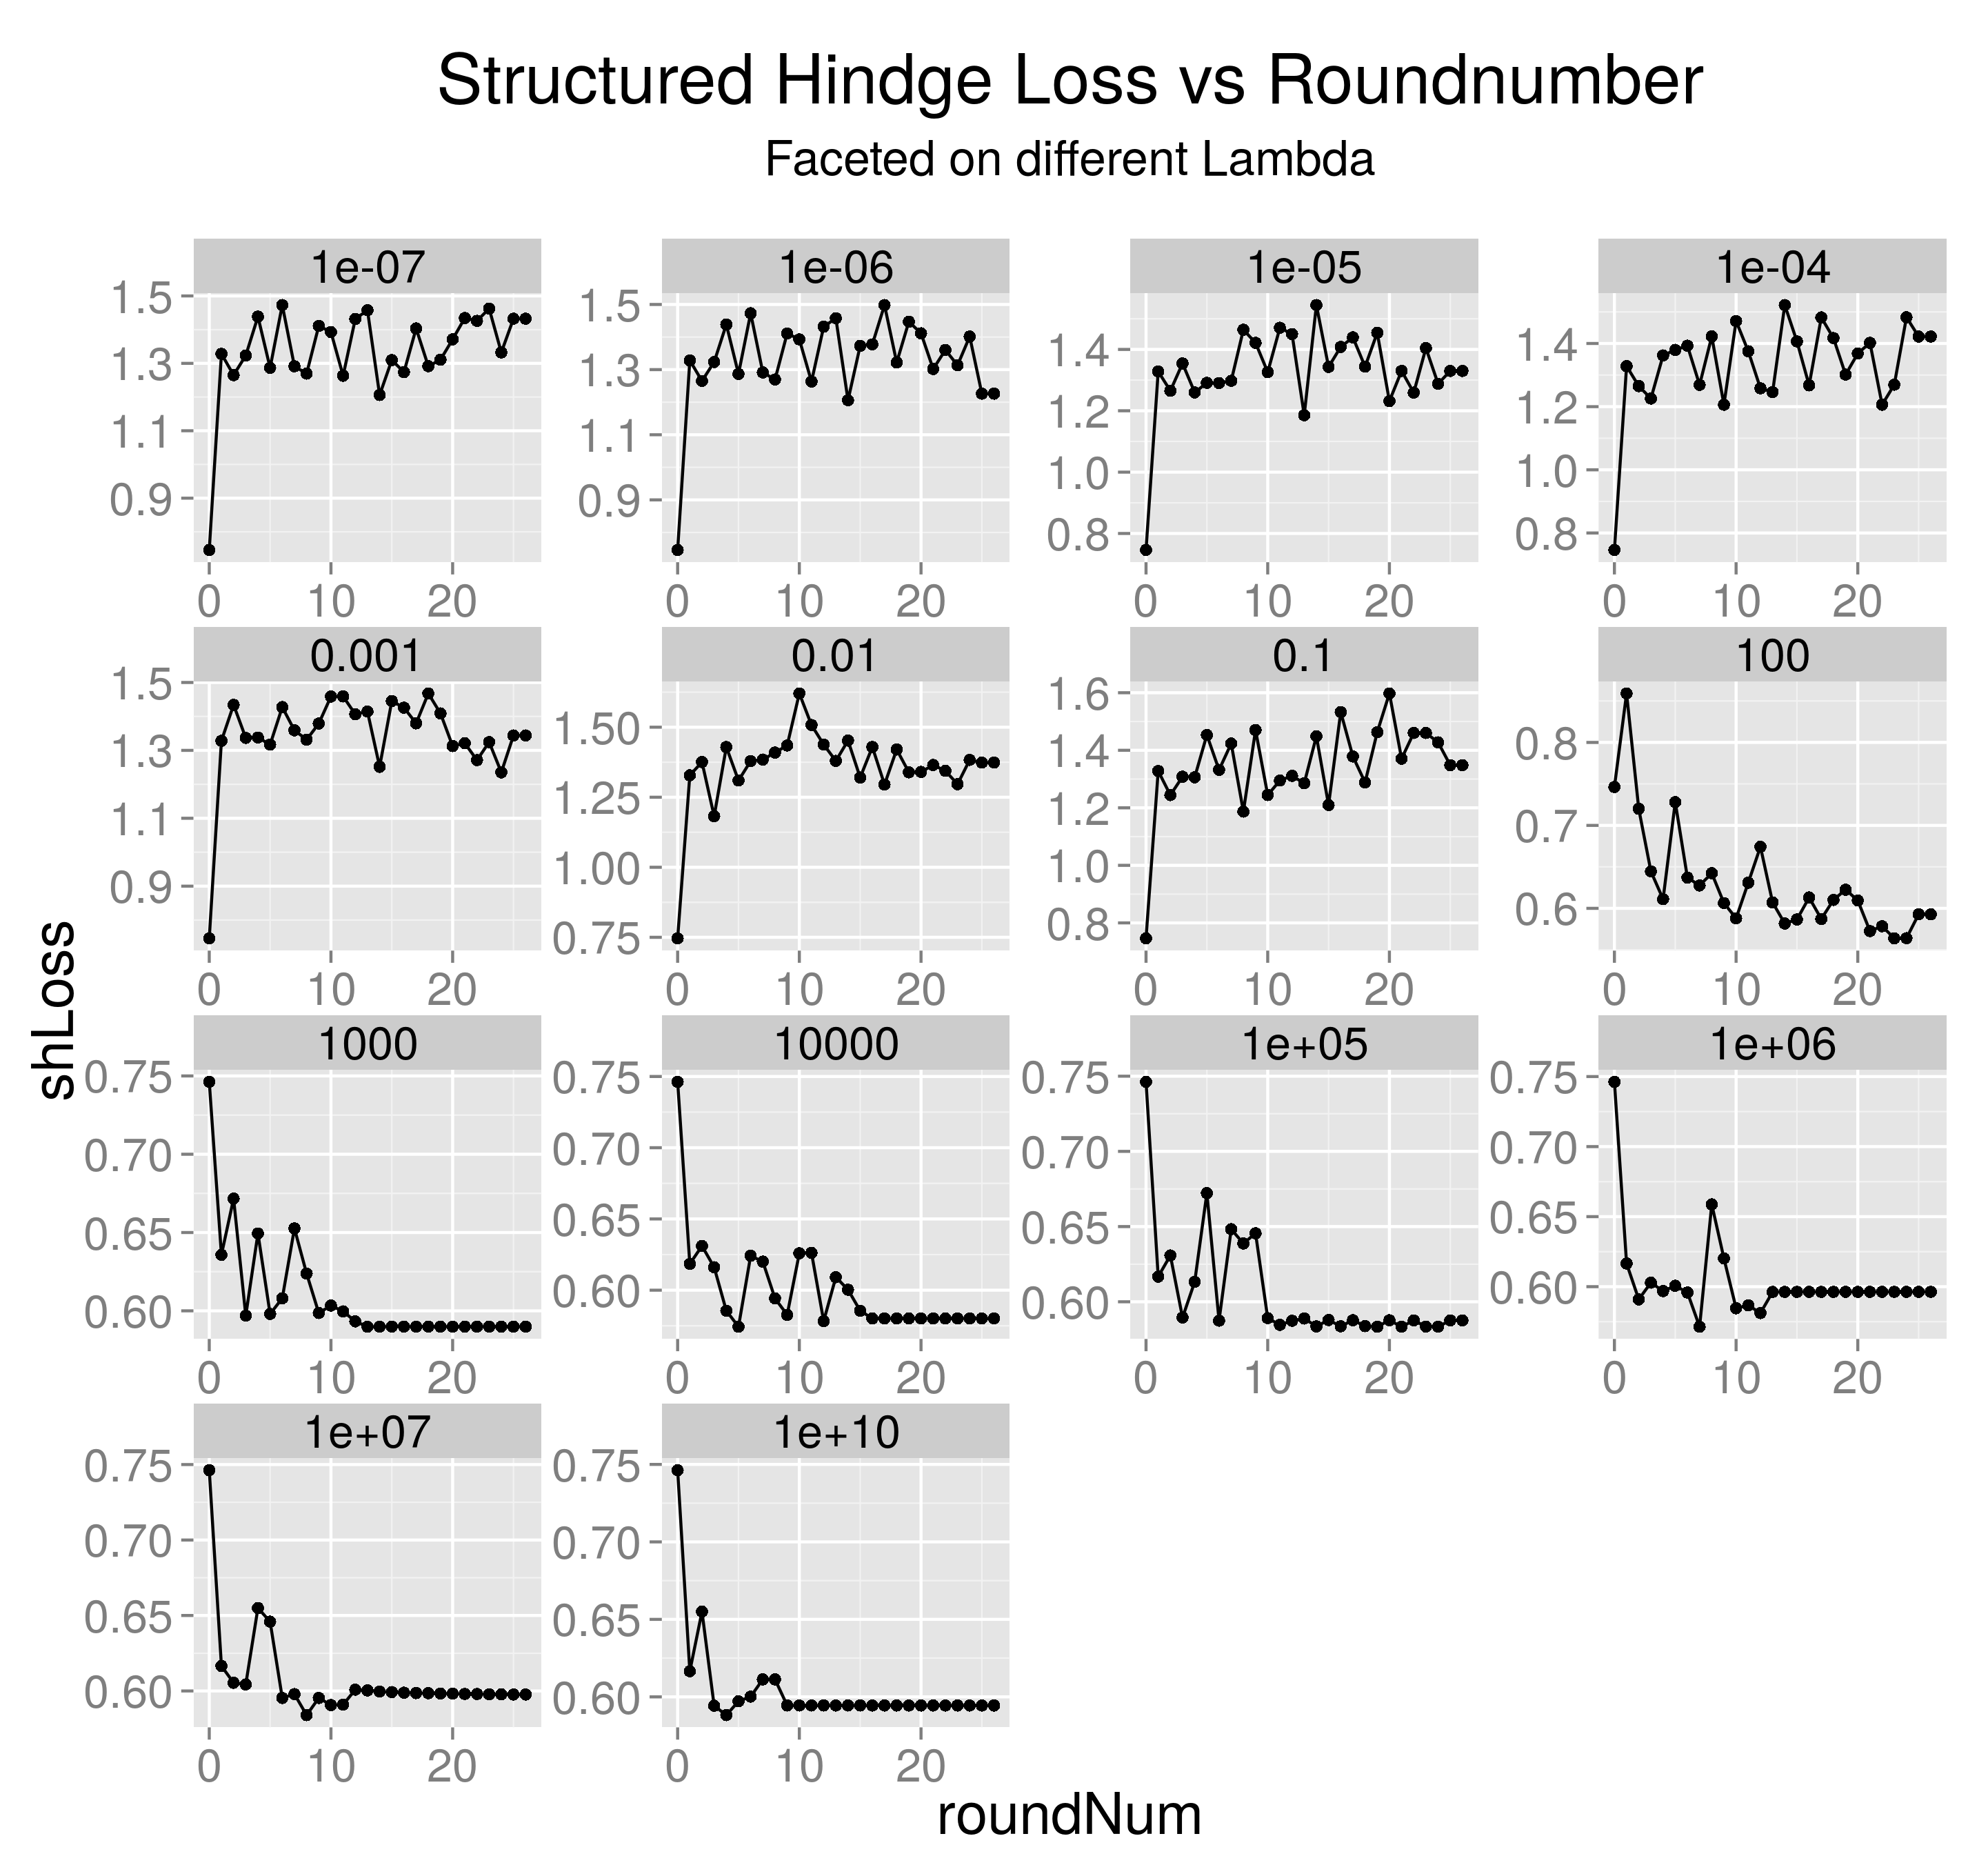
\includegraphics[width=0.8\textwidth]{images/structuredHindgeLoss_vs_lambda_per_Round_msrc_subset.png}
  \caption{This Figure shows the Structural Hinge Loss $\shlossexp$ over time varying the regulerization paramater lambda.  A clear difference can be seen between low lambdas up to 0.1 which do not have a negative trend and also do not seem to converge in terms of structured hinge loss, while lambdas 100 and above have a clear negative trend over time and as lambda gets larger they also converge faster. It should be noted that each experiment starts with the same $w$ and hence also starts with the same structured hinge loss of 0.7462. Data( MSRC version 2 \cite{msrcDataSet}) 	 } 
  \label{fig:lambda2}
\end{figure} 

\begin{figure}
  \centering
  \figuretitle{ Test Error vs Lambda, Using Standardized Features}
  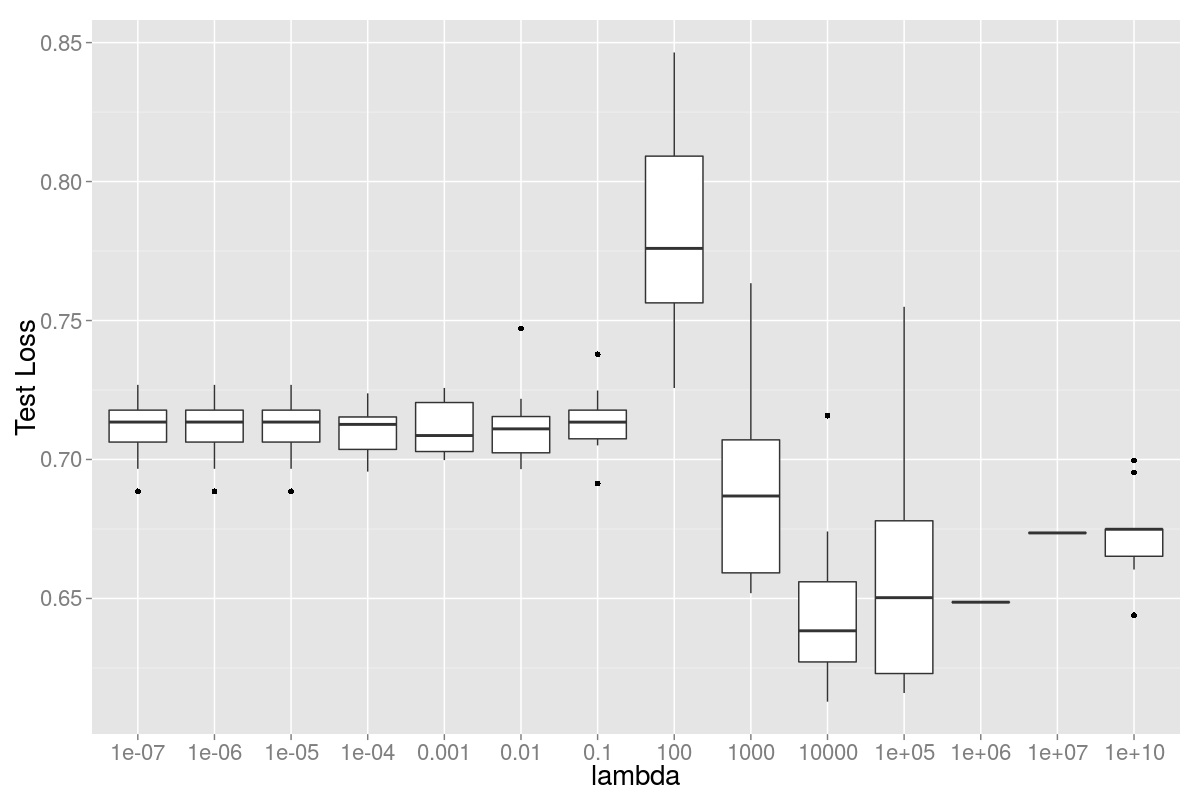
\includegraphics[width=1.0\textwidth]{images/testError_vs_lambda_msrc_stdON.png}
  \caption{  Similar to Figure \ref{fig:lambda1} we can see that low lambdas do not converge properly and hence have significantly higher loss. In this experiment the lowest loss is at 100000 several orders of magnitude higher than in Figure \ref{fig:lambda1} which ran the same experiment only changing the  feature standardization setting.; Data( MSRC version 2 \cite{msrcDataSet} ) 	 } 
  \label{fig:lambdaSTD2}
\end{figure}
\par
To gain farther understanding about the effect lambda has on convergence we can consider the effect it has on the $norm(w)$ over time. See Figure \ref{fig:lambdaWnormNucl1} which shows us how the norm of $w$  does not converge with a lambda of 100 and below but as lambda is increased we can see the curvature also increases indicating it would converge faster with higher lambdas. The test scores with really low lambda are not good but they are still significantly better than pure chance labeling, this can be explained when considering that as lambda goes to zero the optimization problem becomes a simple structured perception which still has the ability to learn a decision boundary but it of course has very poor generalizability as can be seen by the high variance in the score between rounds in Figure \ref{fig:lambdaTestNucl2}. 
\par
Lambda 1000 has a nice shape showing in early rounds $w$ is changing significantly from its initialization of zero and then the norm increase plateauing indication the model has reached some kind of a stable point. Although the $norm(w)$ can appear to be staying constant while the direction of $w$ changes continuing to improve accuracy. Still since we change $w$ in incremental steps such a curve as with lambda=1000 is indication of a good choice. This choice of lambda can be confirmed if one calculates the test error every round as in Figure\ref{fig:lambdaTestNucl2} and we observe a decreasing trend over successive rounds. 
\par
Lambdas greater than or equal to 10000 make their initial move away from zero in the first round but then steadily decrease until plateauing. One would expect that this strange kind of behavior would not result in any reasonable solution but it turns out if we look at Figure\ref{fig:lambdaTestNucl2} that the test error for the highest lambda is actually very close to the best solution found at $\lambda=1000$. To explain this behavior consider the dual objective $\dualObj$ where $\dualA$:=$\dualAexp$ and  $\dualb$:=$\dualbexp$, with very high lambdas the first term of the dual would drop out due to the squared $\dualA$ with a $\lambda$ in the denominator ( $\dualObjLimitLambda$). Now we can see that with high lambdas solving the dual would end up optimizing for the point which would have the highest loss for each $\ySpace$ individually such that $\alpha_i(y^\ast)=1$ where $argmax_{y^\ast}\lossFn(y^\ast) $ and $\alpha_i(y^\prime)=0, \forall y^\prime \neq y^\ast$ since $\alpha$ is constraint with $\dualObjConst$. With KKT conditions $w=\dualA \alpha$ is simply the sum of the joint features maps of the most violating label configurations for each datapoint. If we where to consider this solution in the special case of the binary SVM $w$ would be the vector which if extended would go through the centroid of both classes. The figures used in this section where based on data which was infact binary \cite{ucsbData} and if we look at Figure \ref{fig:lambdaSTD2} which used the MSRC dataset with 24 labels the high lambda solutions are much farther away from the optimal than with binary labeled data.
\par




\begin{figure}
  \centering
  \figuretitle{ Norm(W) over rounds, faceting Lambdas}
  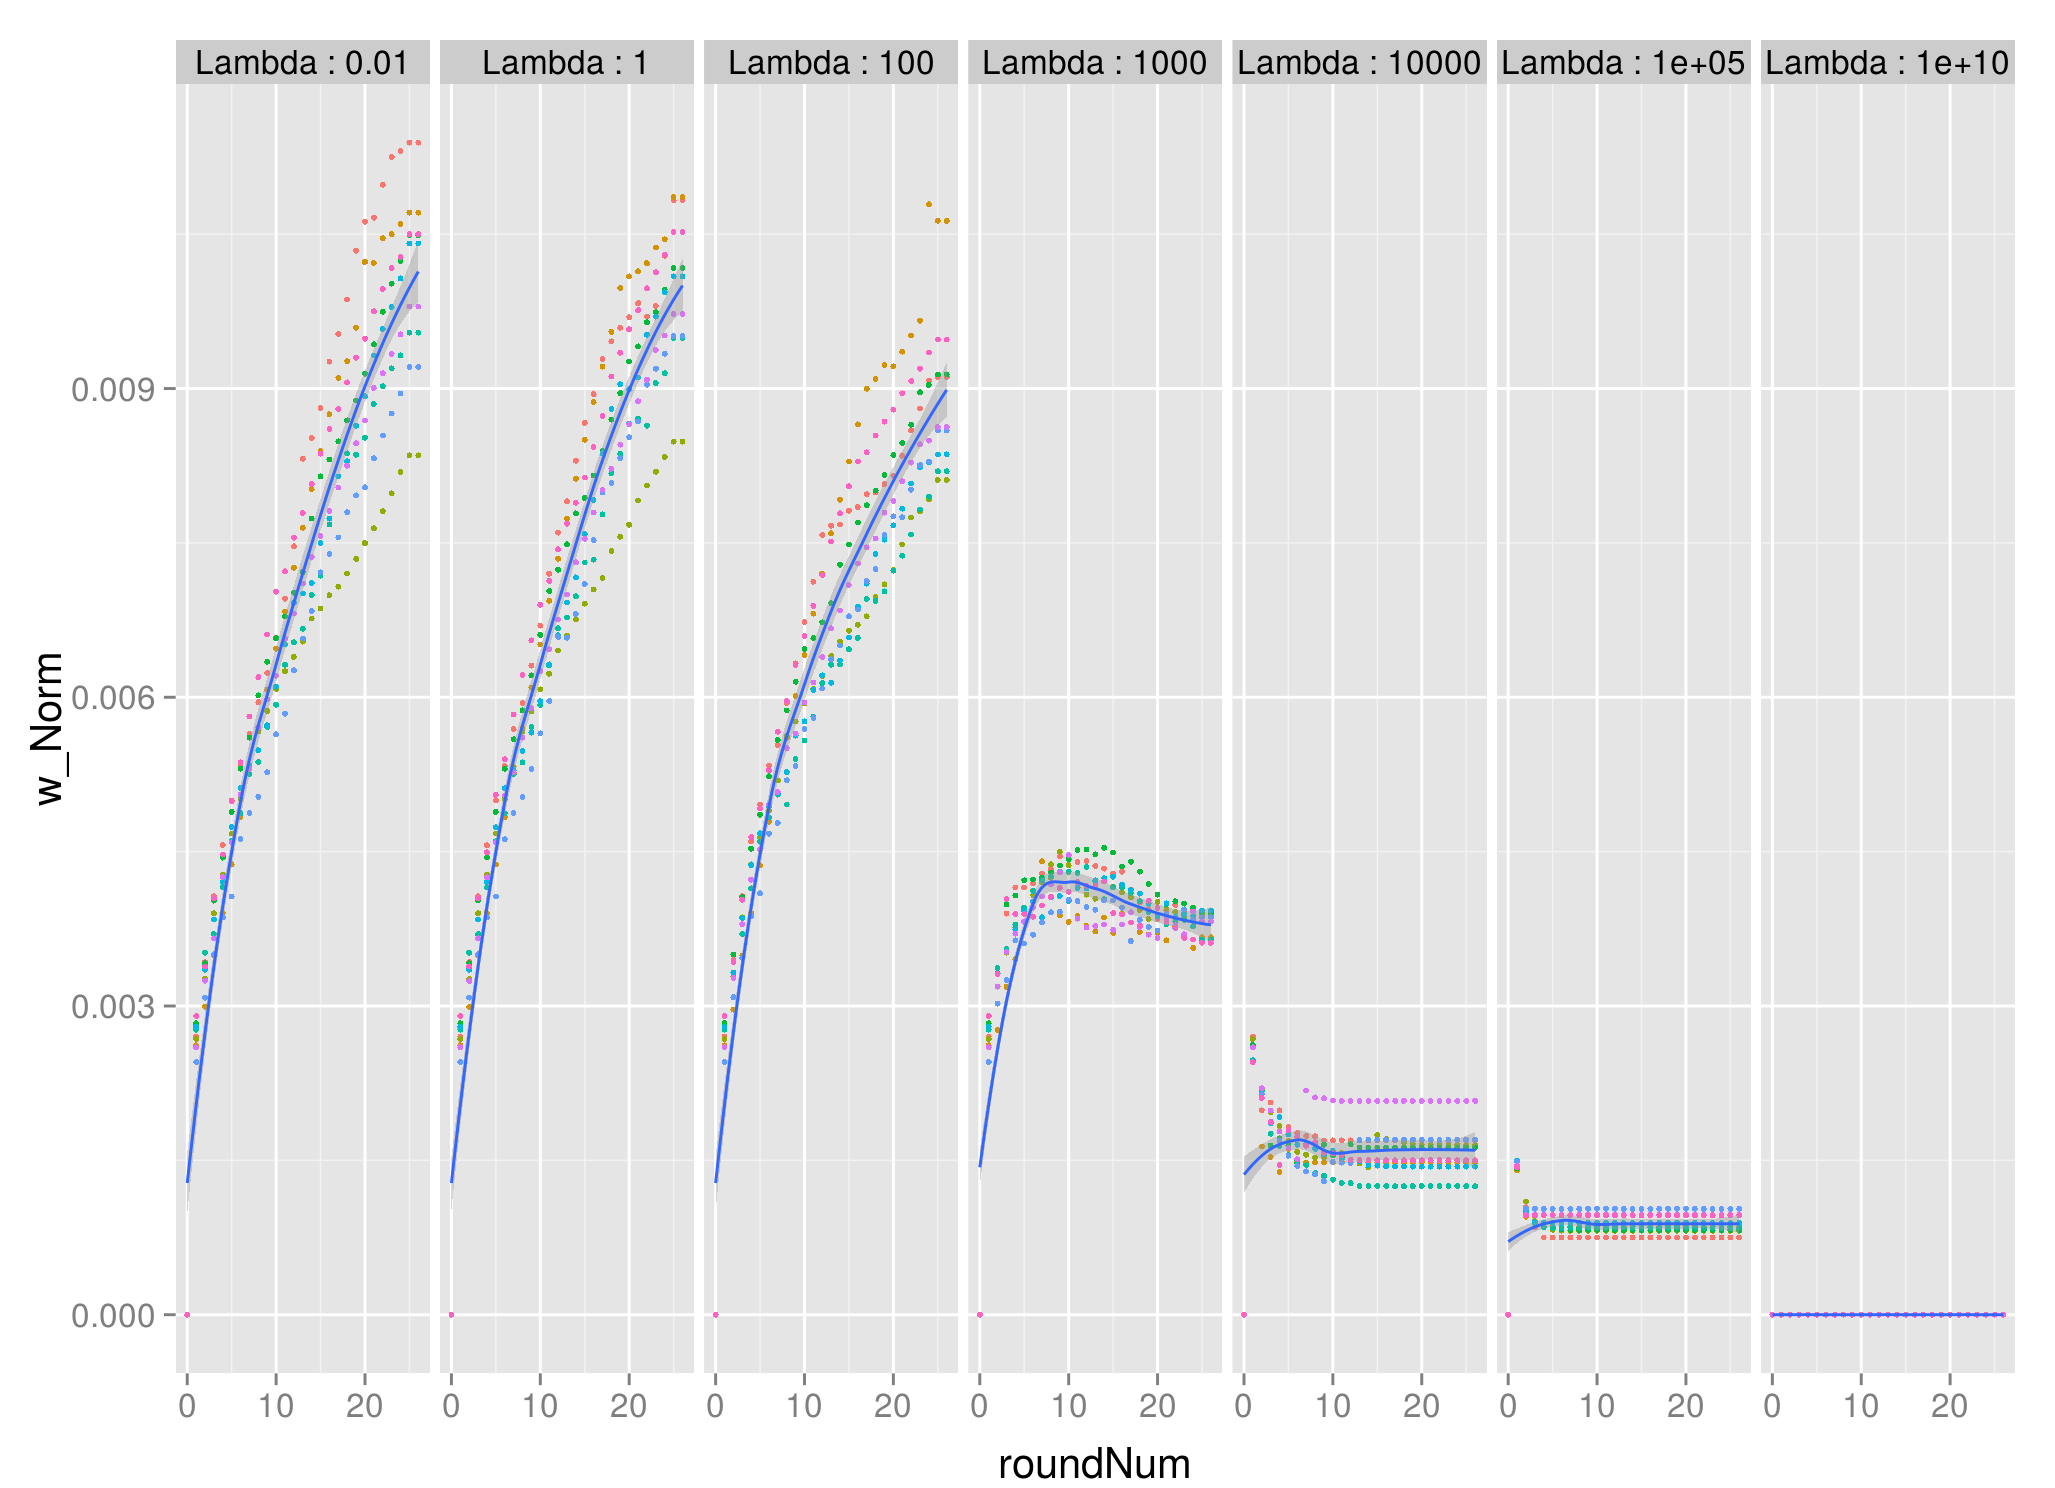
\includegraphics[width=1.0\textwidth]{images/wNorm_nuclei_equalScale.png}
  \caption{ The change in the Norm of the weight vector $\weightVec$ over time is a good indicator of the algorithms convergence depending on lambda. When Lambda is 1 the augmented hinge loss will prefer the $\weightVect$ which has the smallest amount of loss, once the loss can not be improved significantly anymore it will start to choose $\weightVect$ with a larger margin (Large Margin and Low Norm are equivalent in the SVM). The smaller $\lambda$ gets the longer the algorithm can optimize the loss without worrying about the margin. If Lambda where zero then we would have a simple perceptron. When lambda becomes too large the norm curve of $\weightVect$ does not have the expected trend but one can still see if the algorithm converged. Data( Single Channel 3D Nuclei \cite{ucsbData}) } 
  \label{fig:lambdaWnormNucl1}
\end{figure}

\begin{figure}
  \centering
  \figuretitle{ Test Error over rounds, faceting Lambdas}
  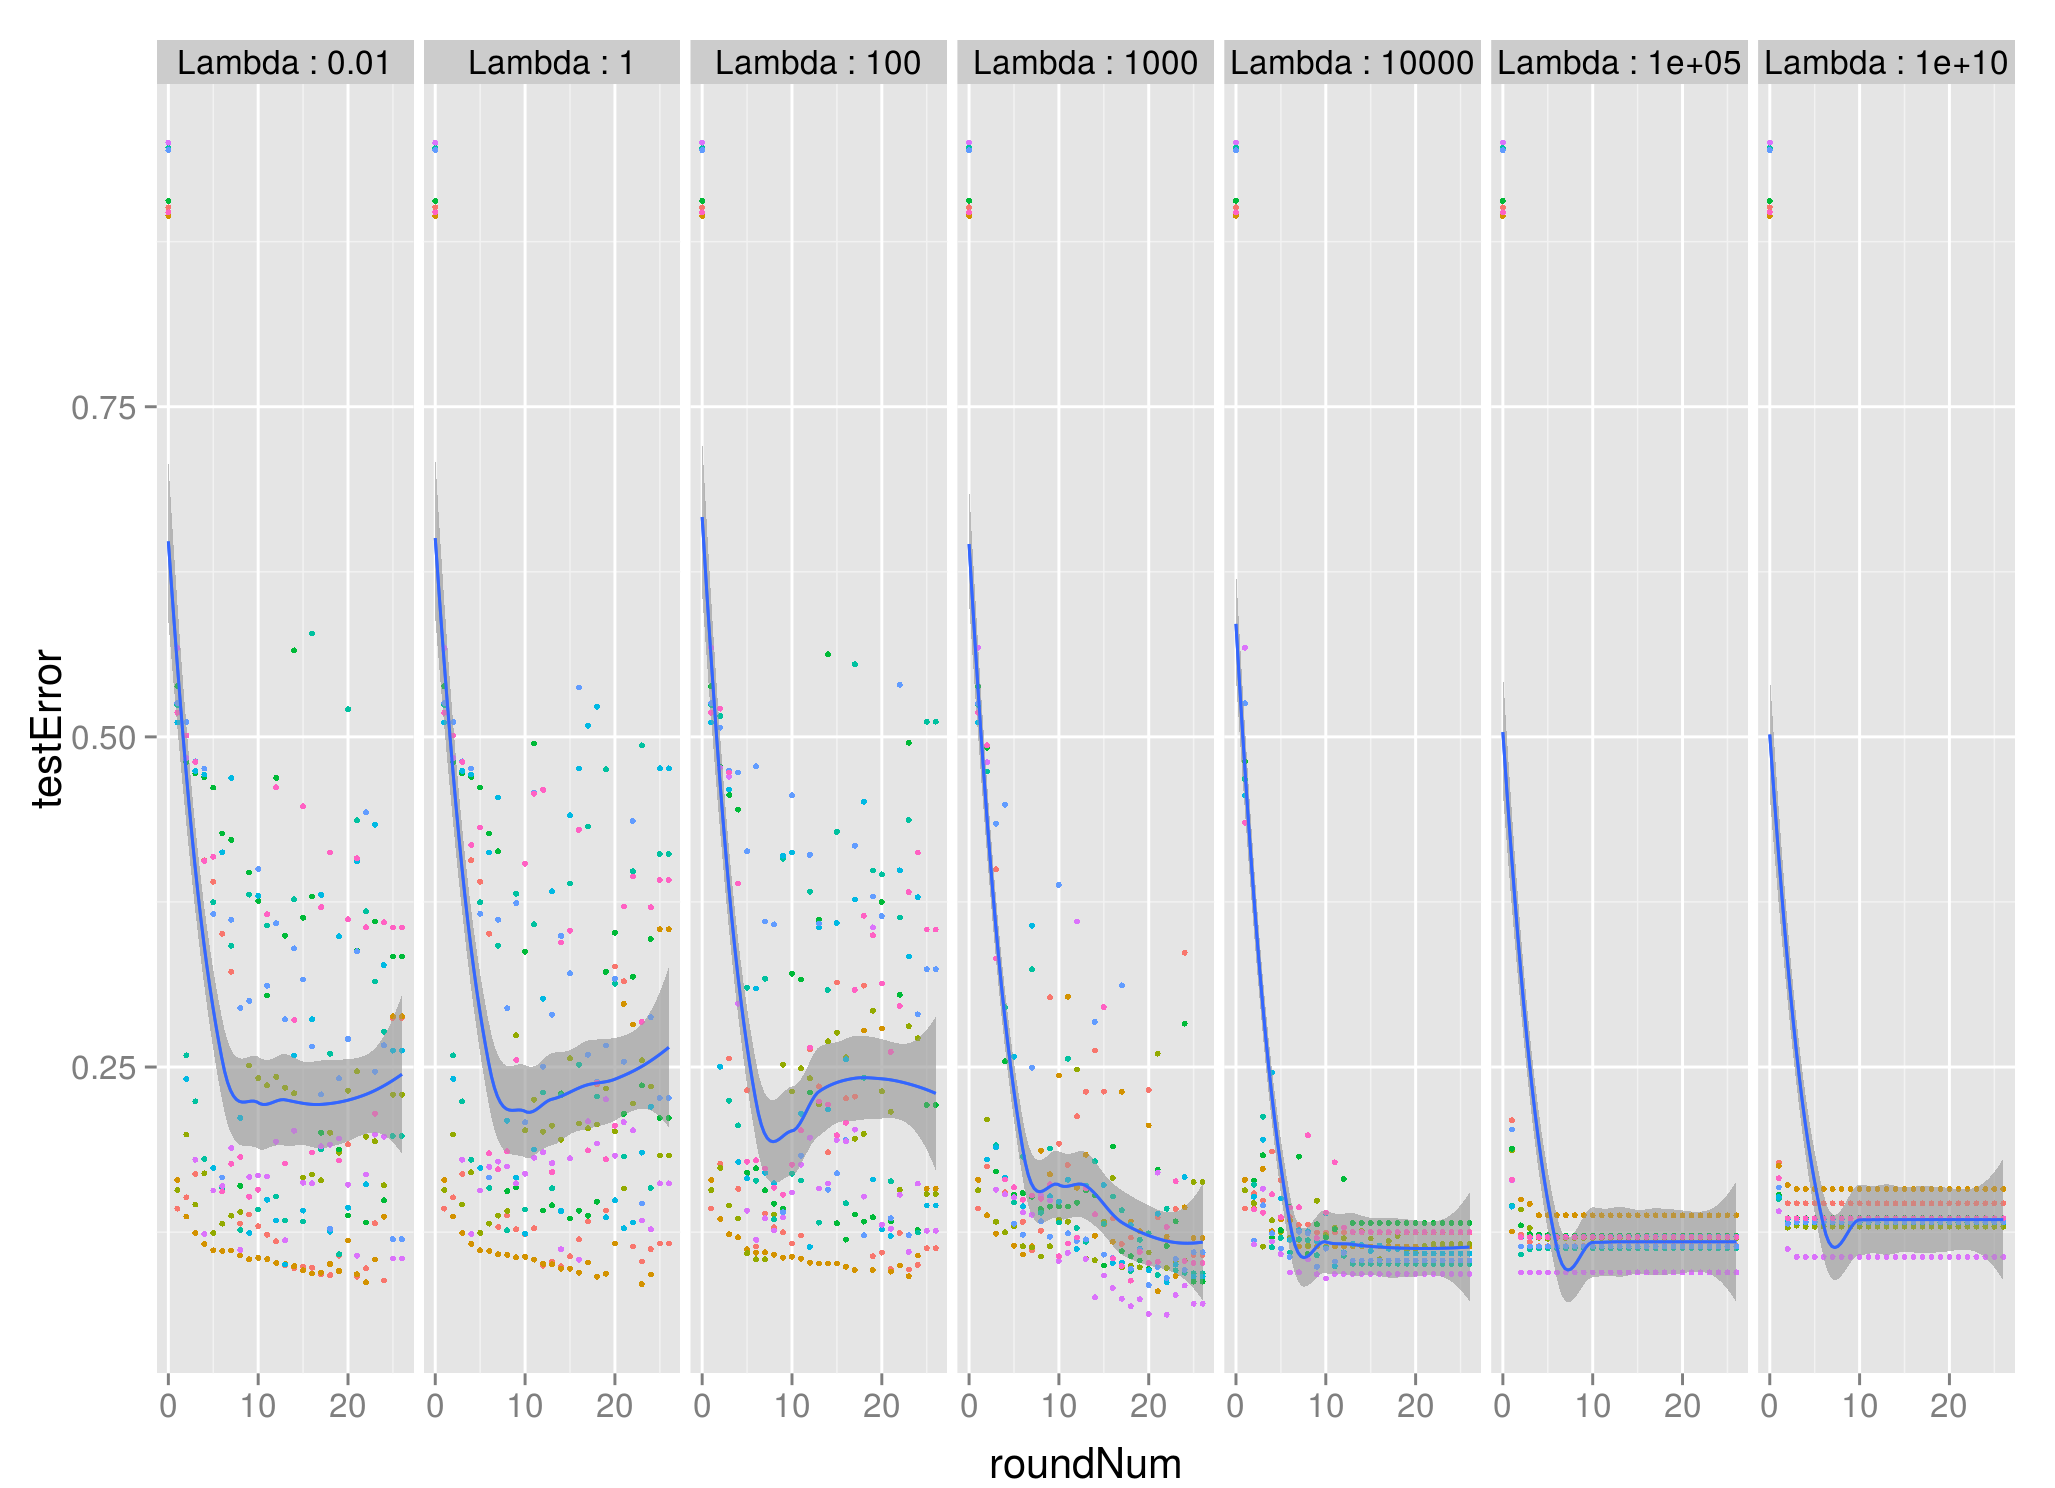
\includegraphics[width=1.0\textwidth]{images/testLoss_nuclei_equalScale.png}
  \caption{  Looking at the curve of Test Error over time with different lambdas we can see that higher lambdas converge faster and if one sets lambda two low it does not seem to converge at all. Data( Single Channel 3D Nuclei \cite{ucsbData})} 
  \label{fig:lambdaTestNucl2}
\end{figure}


\section{Data Dependent Pairwise models}
To examine farther why the data dependent models did not outperform the standard pairwise model we plot the convergence rate of the pairwise indexes of $w$. As seen in Figure \ref{fig:mitochonPairwiseNorm} the curve of the norm of $w_{pairwise}$ over sequential rounds is much steeper for the standard pairwise model as compared to the two data dependent models presented. This indicates that the data-dependent pairwise terms may have needed more rounds to converge than simple pairwise model. A rational for the difference in convergence rate could be that the data dependent term can only gain information from the portion of the transitions which are binned into that group of the data dependent pairwise model hence it probabilistically requires more data to gain the same amount of information in each bin. To test this hypothesis we reran this experiment with larger suboptimal lambda selections. In Figure \ref{fig:mitochonDifLambdaShLoss} we see the Structured Hingle Loss over time and as the lambda gets higher there is a trend of the data dependent models improving their gain over the simple pairwise model. indicating that the data dependent pariwse term could converge better with a higher lambda value but such high lambdas result in lower Test Error due to the unary term as described above. Preliminary results with high number of rounds $\geq 110$ show the data dependent models starting to converge and improving the test error over simple pairwise models. Put since the unary term does not require this many rounds to converge we purpose an addition to the current system which would allow for different regularization of the pairwise term seperatly from the unary term. 




\begin{figure}
  \centering
  \figuretitle{ Pairwise W norm over Sequential Rounds}
  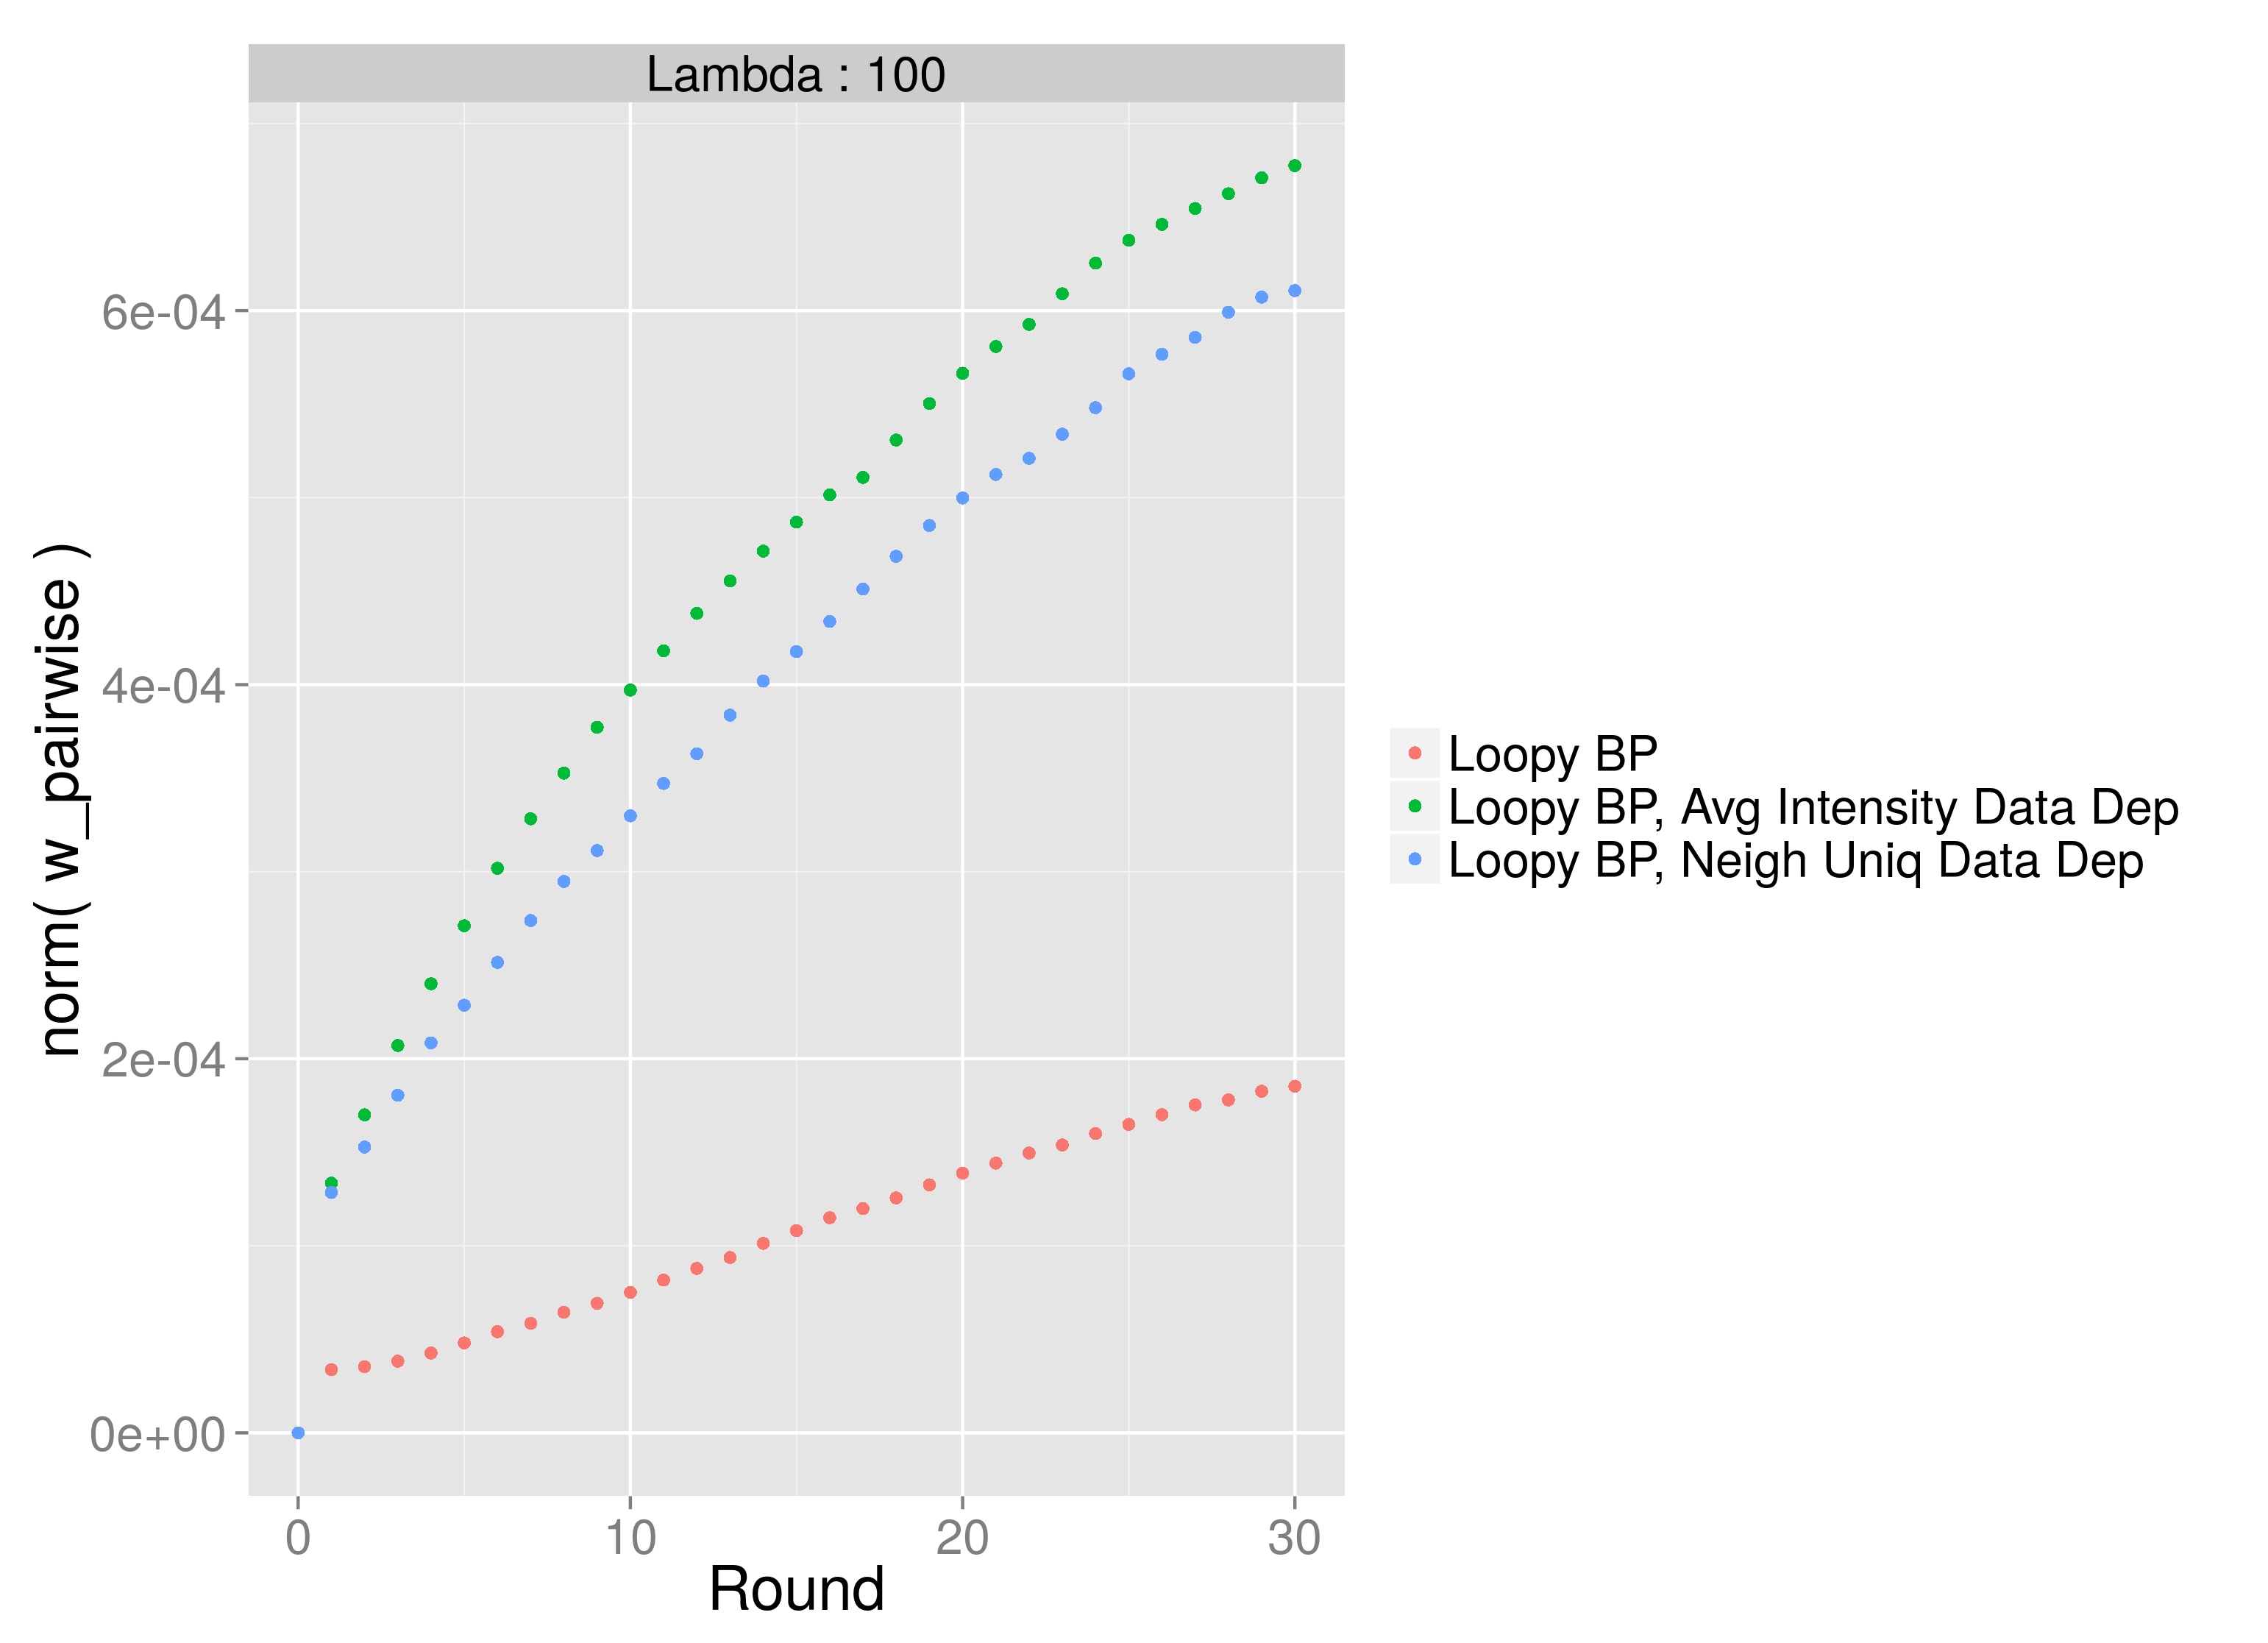
\includegraphics[width=0.8\textwidth]{images/mitochonSplit_pairwiseWnorm_overTime.png}
  \caption{ The above graph displays the norm of the pairwise portion of the weight vector. The weight vector is always initialized to zero at round zero. The curve of the norm of $w$ can indicate convergence behavior. In this experiment it appears that Loopy BP (the Simple Pairwise model) is converging faster than both data dependent pairwise models. Data:( EM Mitochondira Labeling split into $82^3$ cubes with super-pixels of size $S=10$ \cite{mitochondriaData} )} 
  \label{fig:mitochonPairwiseNorm}
\end{figure}

\begin{figure}
  \centering
  \figuretitle{ Structured Hinge Loss over Time, including Linear Trend Line }
  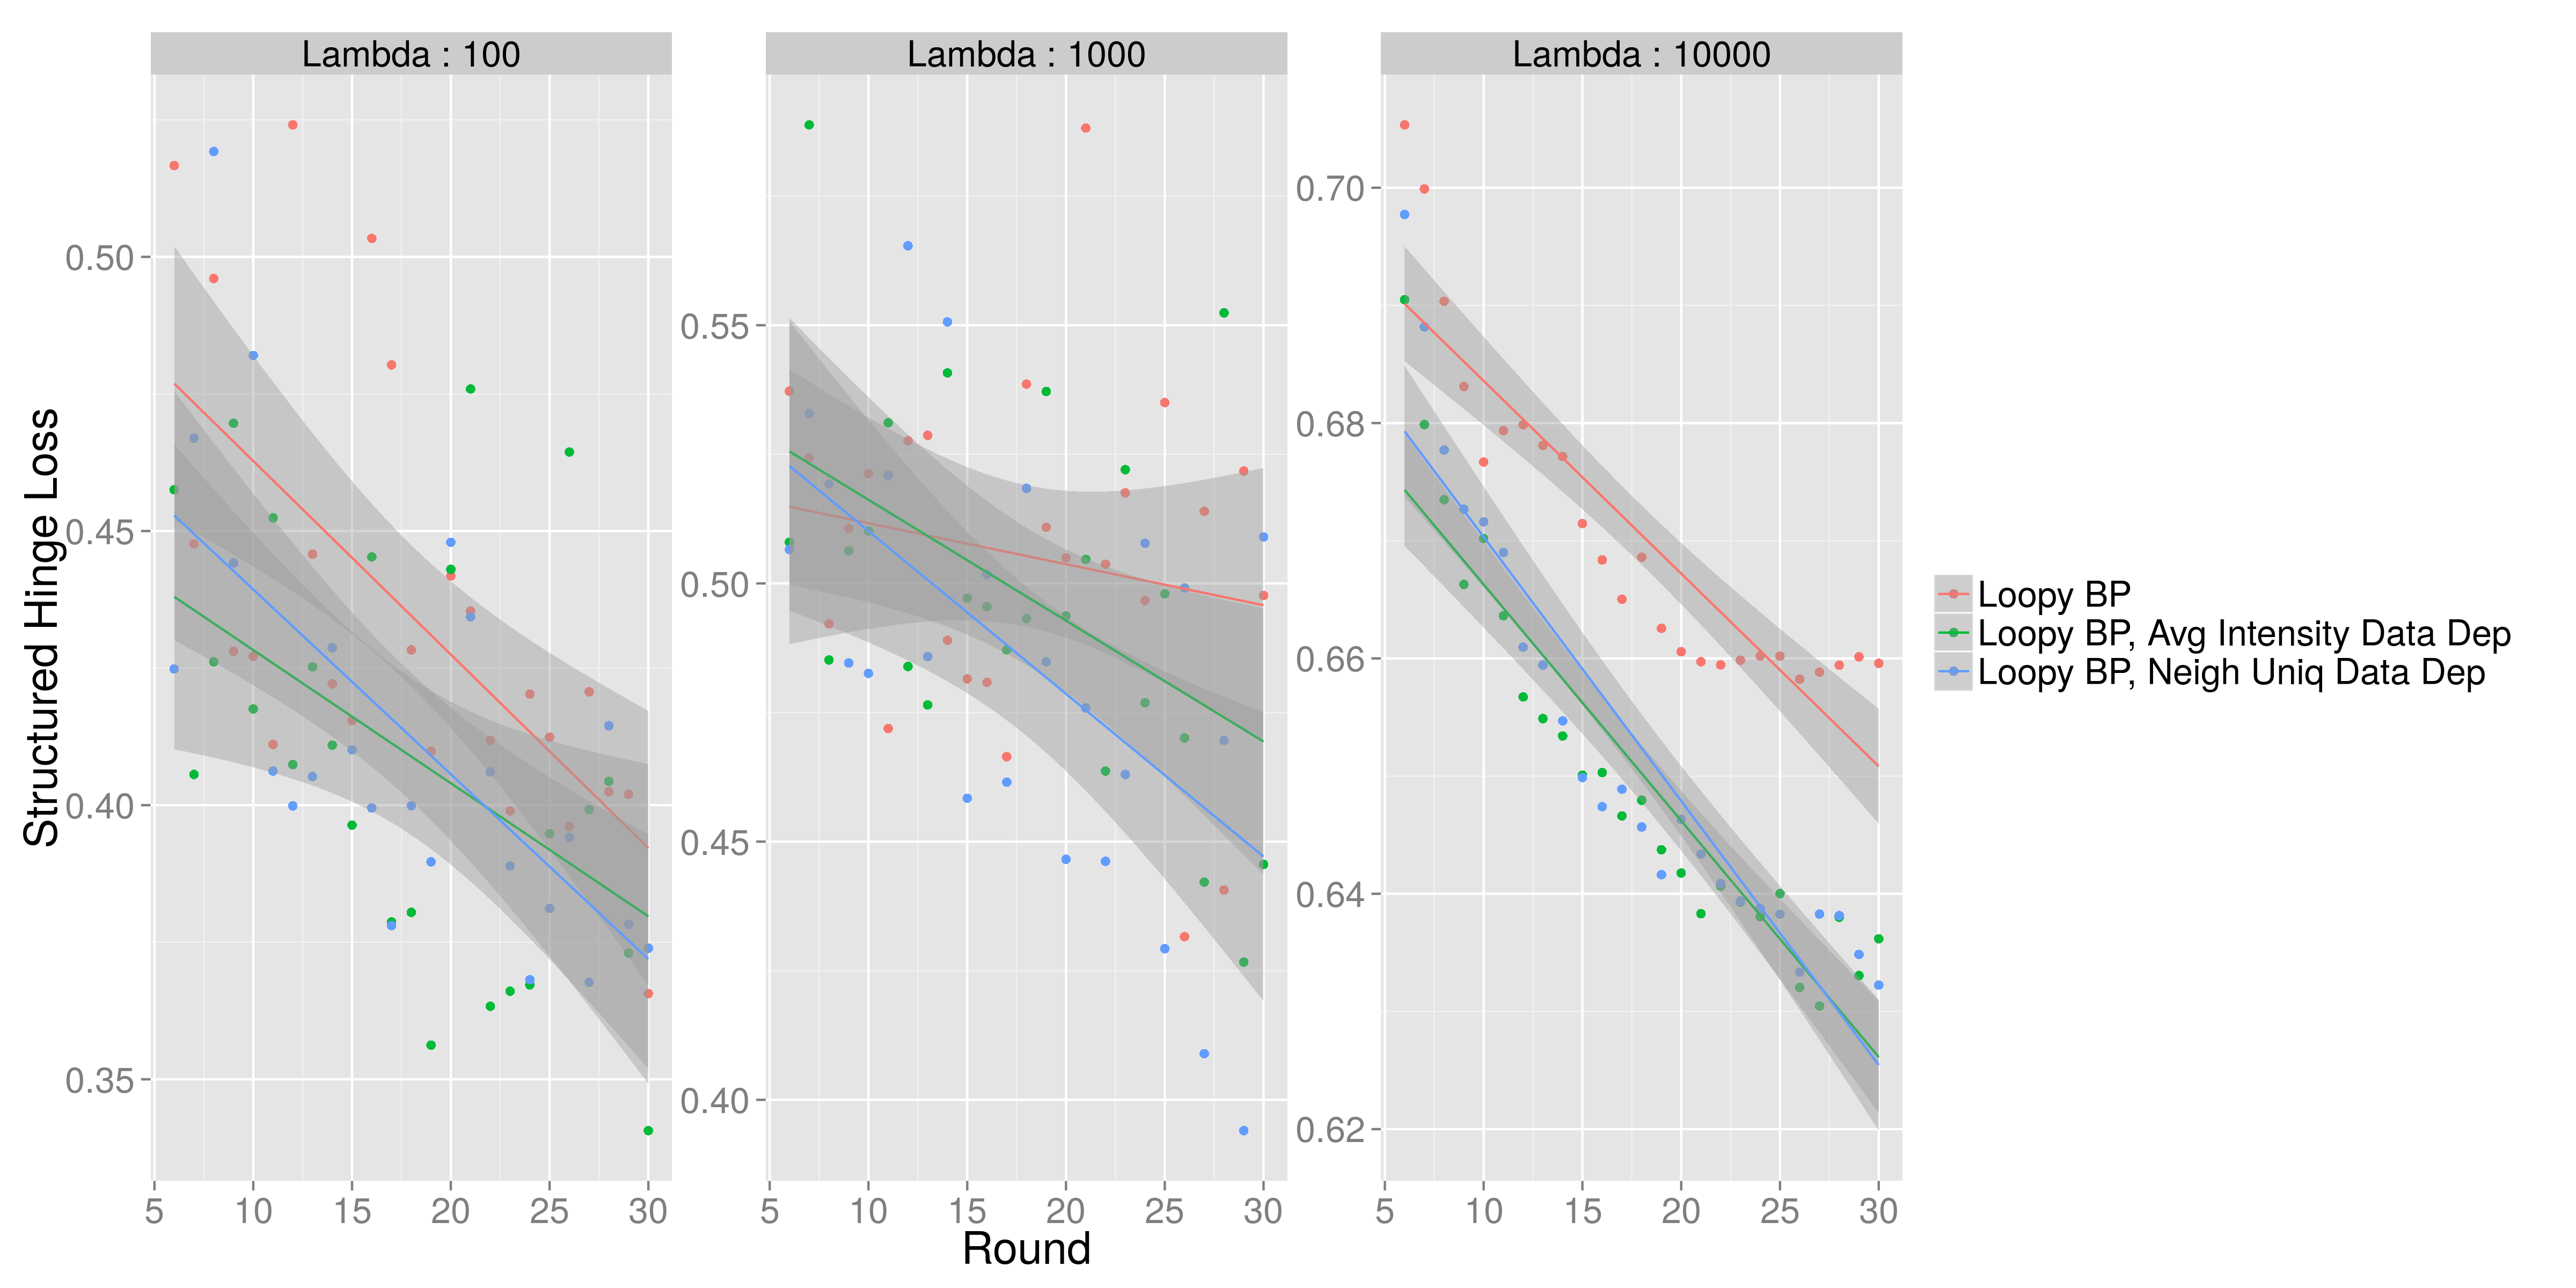
\includegraphics[width=0.8\textwidth]{images/mitochonSplit_shloss_difLambda.png}
  \caption{  This Figure displays the Structured Hinge Loss ($\shlossexp$) over time of the different pairwise models. With the added linear regression line we can see that as we increase Lambda the difference between the simple pairwise model to the data dependent models increases. Higher lambdas cause faster convergence hence we conclude that data dependent models require more rounds to converge. Data:( EM Mitochondira Labeling split into $82^3$ cubes with super-pixels of size $S=10$ \cite{mitochondriaData} )} 
  \label{fig:mitochonDifLambdaShLoss}
\end{figure}




%%%%%%%%%%%
%
%
%
%
%
%
%
%
%
%
%
%
%
%
%
%
%
%
%
%%%%%%%%%%%





\chapter{Distributing Workload}
The dissolve framework which we used to solve the SSVM was written with distribution in mind by 

\section{Single Node, Multiple cores}
Spark can be used to distribute the inference work over a cluster but also it utlizes local parallelization without writing multi-threaded code. In some computing environments it may be cheaper to use one 36-core machine versus nine 4-core machines, or it could be advantageous for the user to avoid time lost in network synchronization.  When distributing on one machine one must consider memory limitations, by default spark assigns 512mb per driver hence if one is running a 36-core machine other than the ram needed for the driver it must have 18432mb available for all the executors. When using \codeInLine{sbt run-main ch.ethz.dalab.dissolve.examples.neighbourhood.runReadTrainPredict } to start the local job one can specify the internal driver memory used with the \inputArgs{spark\_driver\_memory} which should be specified as a string just as in the spark config. 
\par
As is typical when distributing we do not get perfect scaling as adding more executors requires more synchronization work. Figure \ref{fig:singelNodeScale} shows total training time required for the MSRC dataset on a 8 core machine varying the number of local-spark-executors. 
Even when setting the number of executors equal to the total number of cores available we did not observe any thrashing but rather still saw a slight improvement from 7 to 8. Scalling well even up to the max number of cores can be partially attributed to the design where the driver has little work until a round ends and the executor results needto be combined, during this time when the driver is active the executors are ideling. Hence they do not compete for computational resources even when both are on a single machine. The increase in the time needed for the Spark Driver to coordinate the different spark-executors is visualized by the difference between blue and green points (Total Training Time - Theoretically perfect Scaling). From one to two exectuors there is a jump in this difference because this is when merging of results first occurs. As the number of executors increases the distribution coordination time increases but with negative second derivative. Additionally we plotted what training time we would expect if the entire system only needed to run the oracleFn and was being distributed perfectly in Red (Decoding Time / number executors). As expected this curve is slightly above the perfect theoretical scaling because of course the cores of the CPU and the work we do inside the oracleFn are not completely independent. To farter ensure that the oracleFn is being scaled aswell as we think we reran the above experiment with significantly higher loopy belief propagation iterations such that the individual oracle calls are significantly longer. In Figure \ref{fig:singelNodeScaleLonger} we see that under these conditions we get scaling which is even closer to theoretically perfect hence affirming that the oracle calls themselves are very well distributed. 



\begin{figure}
  \centering
  \figuretitle{ Single Node Scalability by Varying Executors  }
  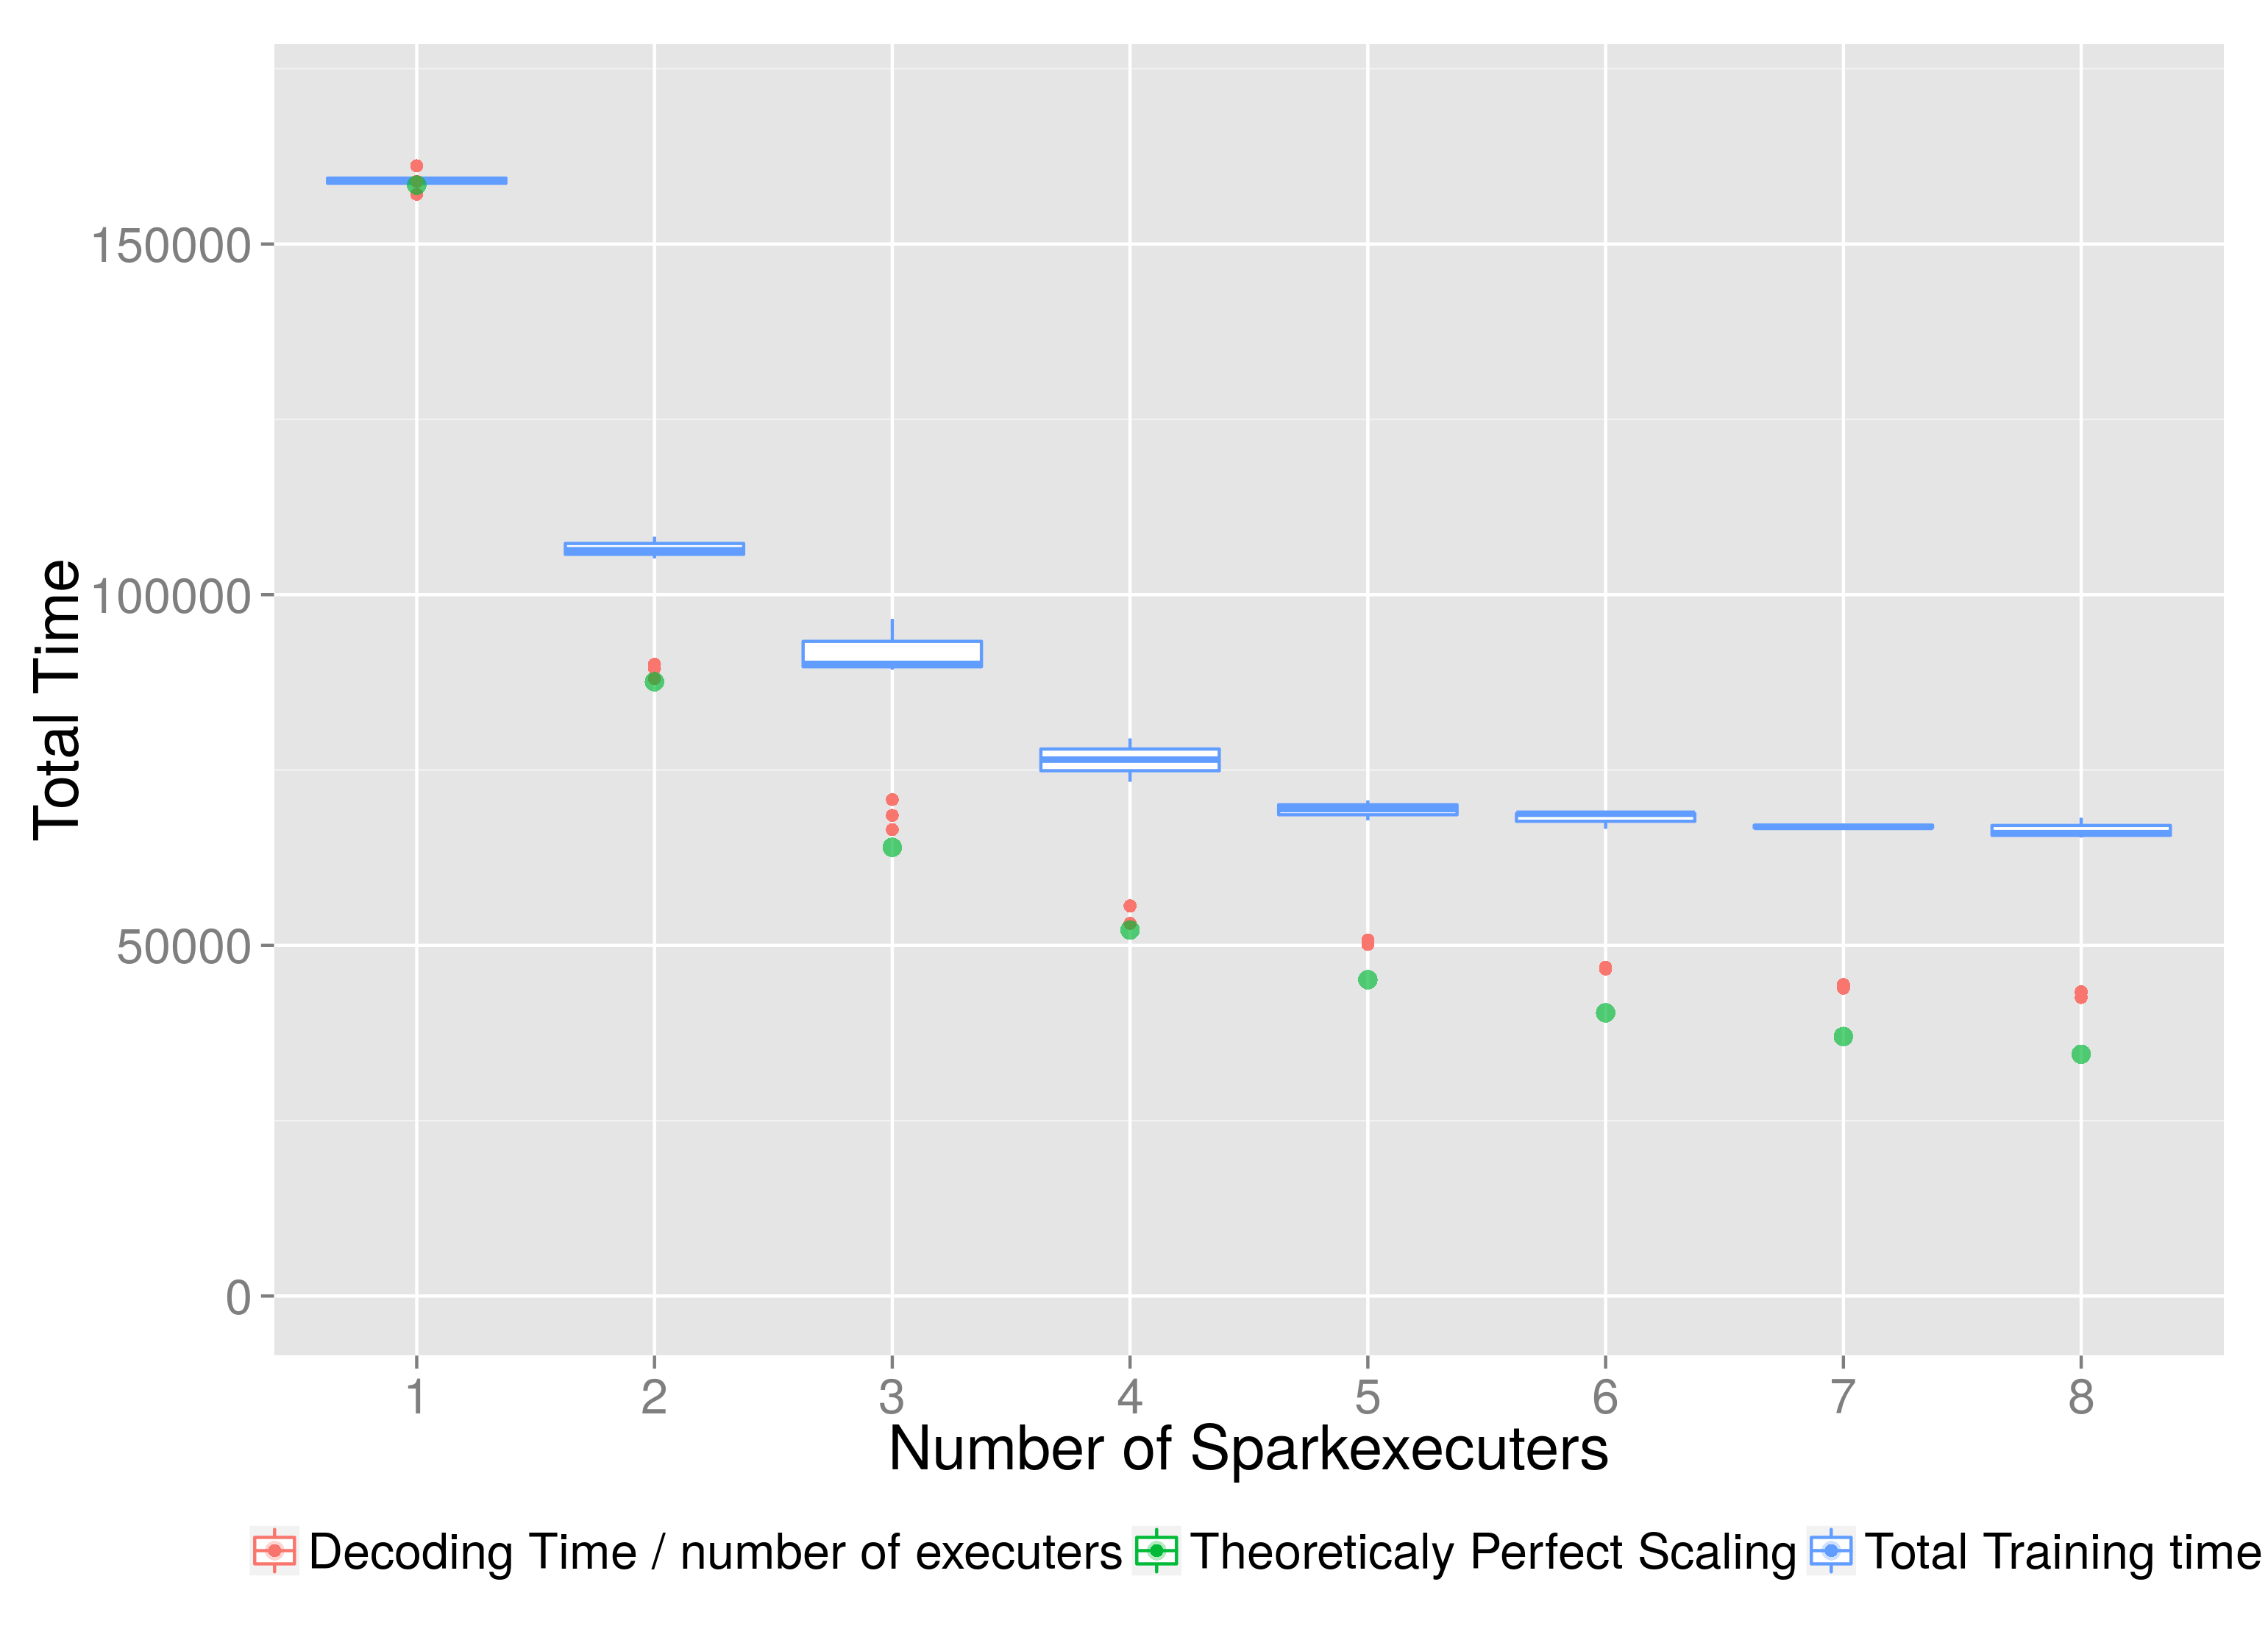
\includegraphics[width=1.0\textwidth]{images/singleMachineScalability.png}
  \caption{ In blue we see the total time to train the model as measured on the driver node, this time consists mostly of time spent in the oracleFn but also there is a constant overhead of ~16000ms and for the experiments with greater than one executor we have a significant amount of work dont on a single thread when combining and coordinating the executors. The red points are the recorded total amount of time spent inside the oracleFn divided by the number of cores available to spark shifted to match the constant overhead of the single executor experiment. The Green points are the theoretically best scaling extrapolating from the pure decoding time of the experiment with only one executor by simply dividing by the number of cores and also shifting the constant overhead.  } 
  \label{fig:singelNodeScale}
\end{figure}
\par 

\begin{figure}
  \centering
  \figuretitle{ Single Node Scalability by Varying Executors (More decoding iterations) }
  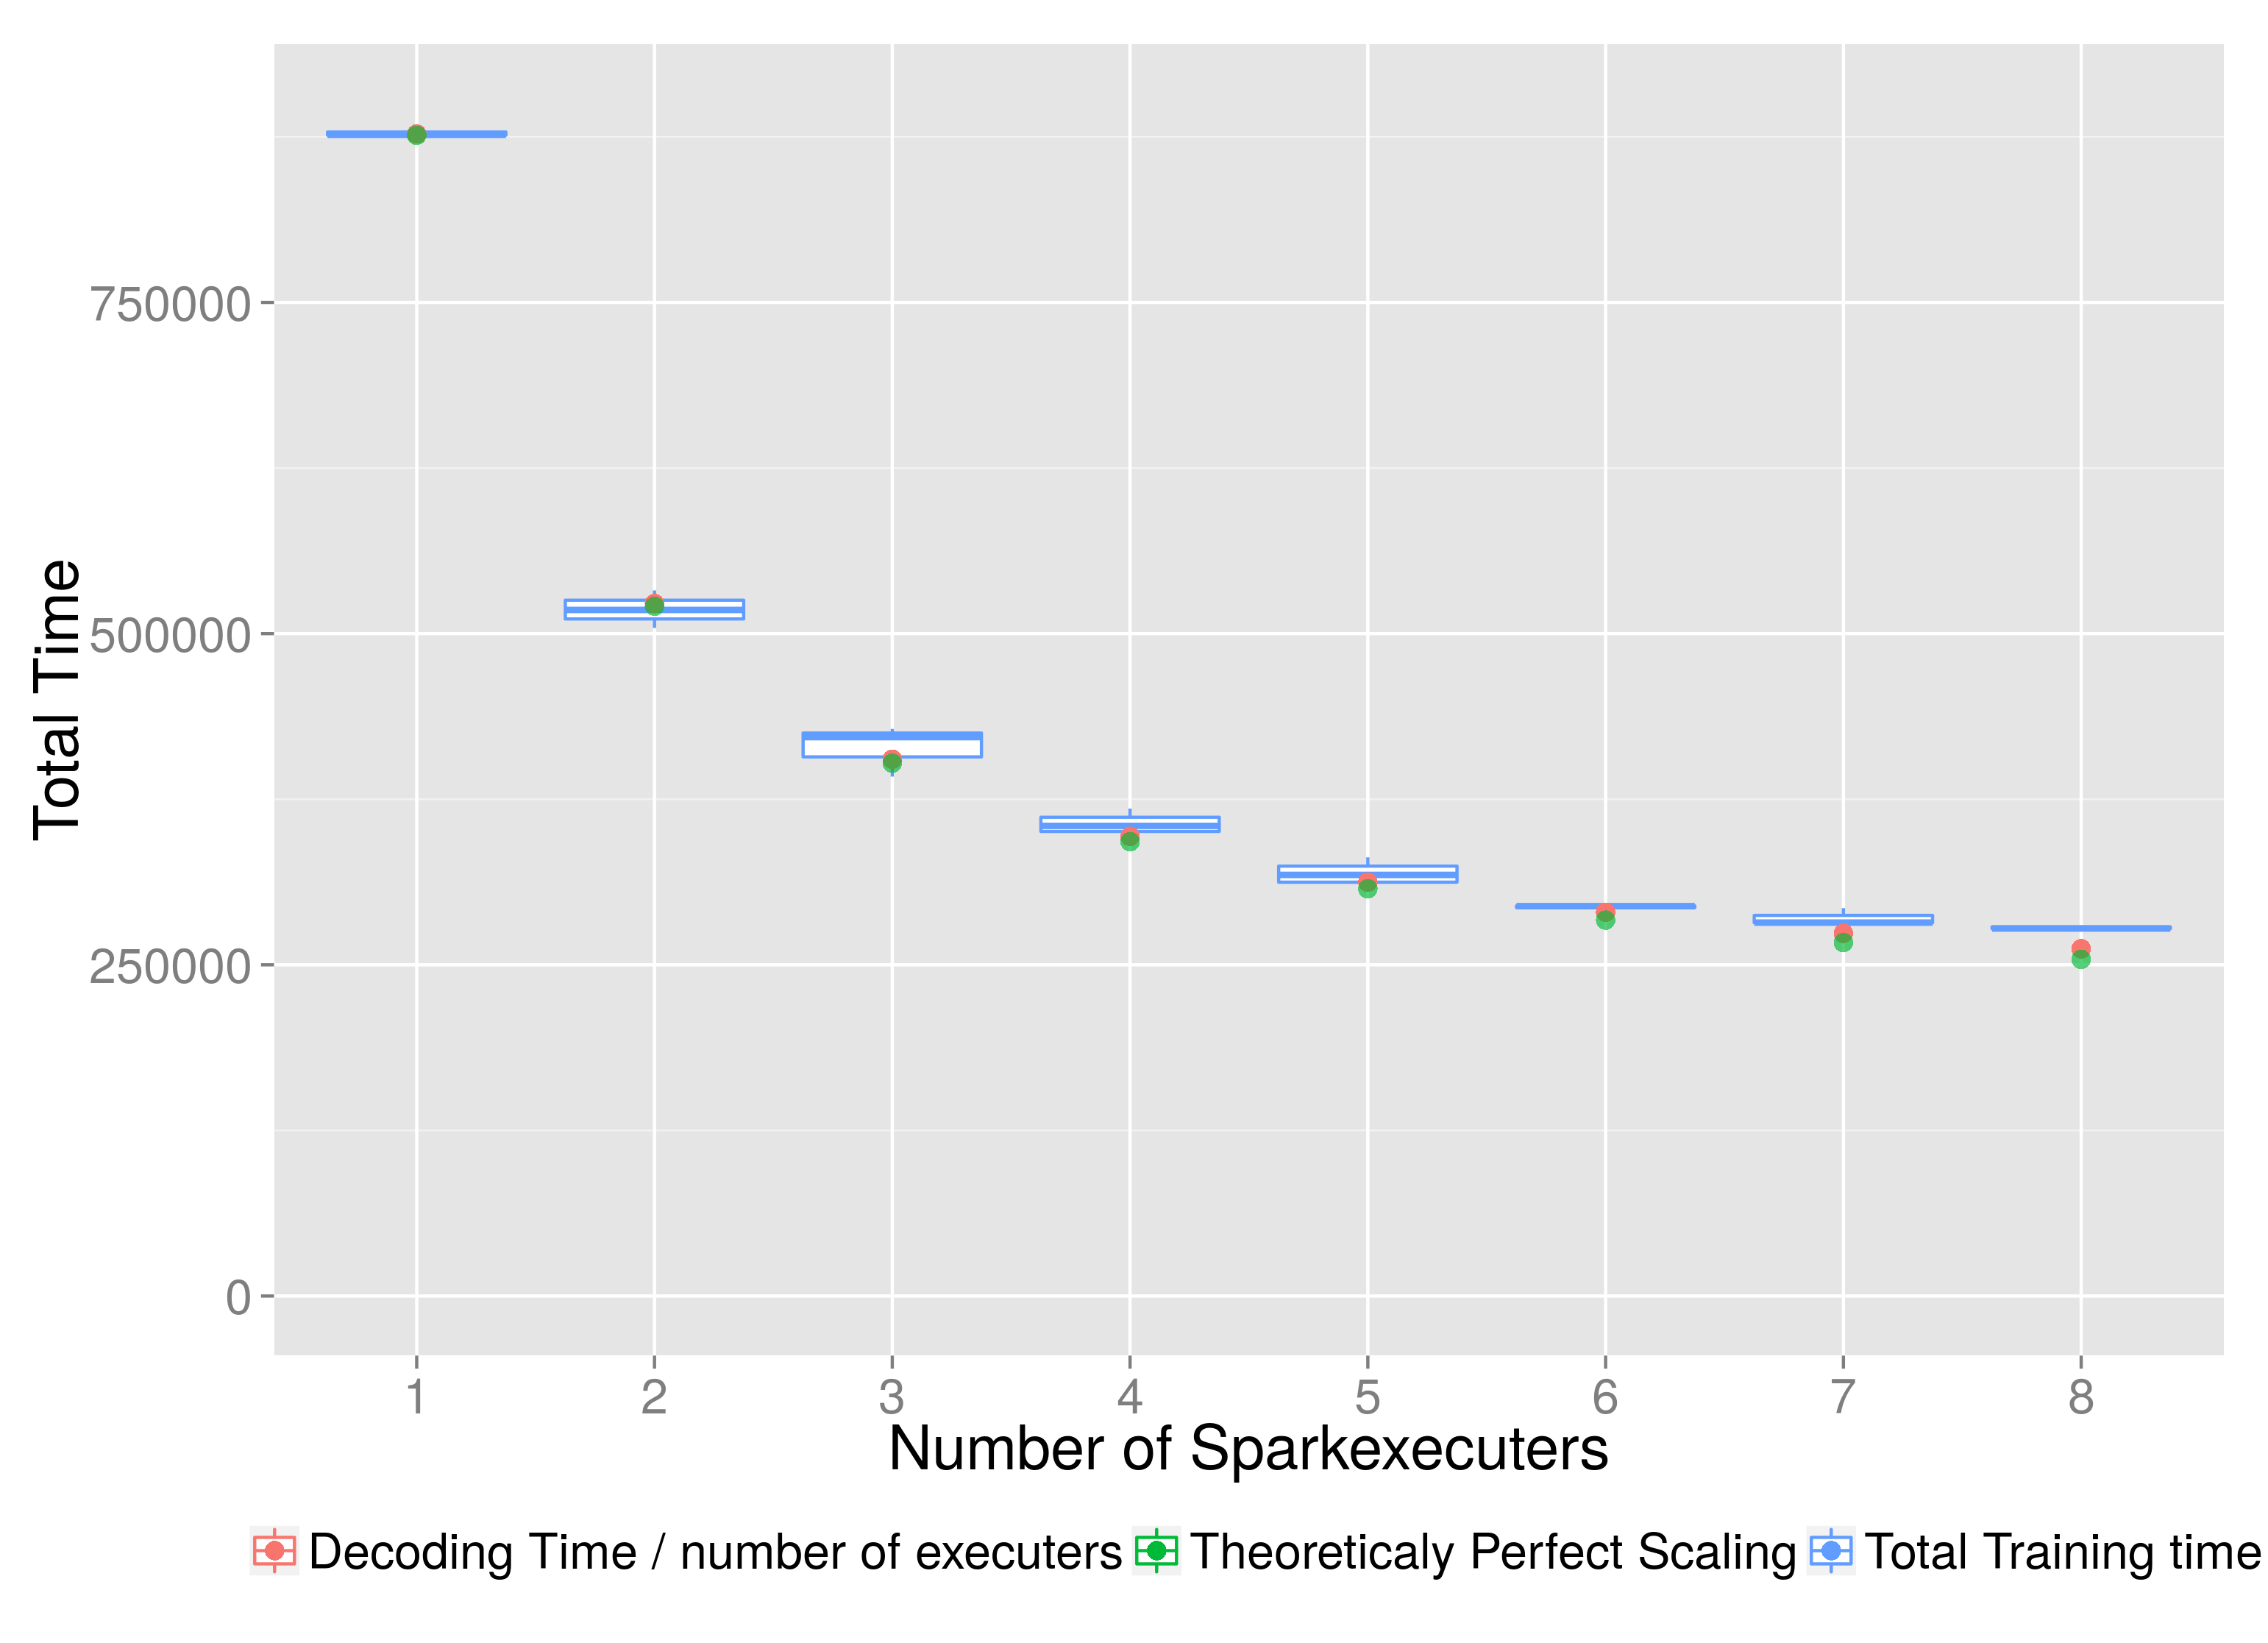
\includegraphics[width=1.0\textwidth]{images/singleMachineScalability_longerDecoding.png}
  \caption{ See description for Figure \ref{fig:singelNodeScale} we reran the same experiment but with more loopy belief iterations to get a more precise max oracle decoding. Comparing to Figure  \ref{fig:singelNodeScale} we see an even better scaling with very little increase in context switching time as seen by the difference to the perfect scaling curve in green. This was expected as we modulated on parameter which only effects the max-oracle timing. } 
  \label{fig:singelNodeScaleLonger}
\end{figure}
\par 

\section{Multiple Nodes, Single core}
As we expected on tasks with a high max-oracle decoding time the additional time required for spark to recombine results over the network does not significantly impact scalability when contrasting to parallelizing on a single machine without network time, see Figure \ref{fig:scaleDistrmsrc1} for details. Additionally the data that needs to be transferred over the network is very minimal because of how dissolve-struct is designed. Dissolve-struct when configure to run Distributed-BCFW utilizes a method optimized for low network traffic called CoCoA (Communication-efficient distributed dual Coordinate Ascent) \cite{cocoa}.CoCoA can be applied to a large class of linear regularized loss minimization objectives, which includes the SSVM image segmentation objective \ref{optimizationFunc}. The primal-dual structure of these problems was used to aggregate partial results from local computations in such a manner that reduced network traffic and avoided conflicts with updates made by different machines. It has also been shown that the CoCoA communication and weight update scheme has little effect on the total amount of computation needed to achieve the same accuracy  as globally communicating methods \cite{cocoa}. 


\begin{figure}
  \centering
  \figuretitle{ Cluster Scalability, Single Core per Machine }
  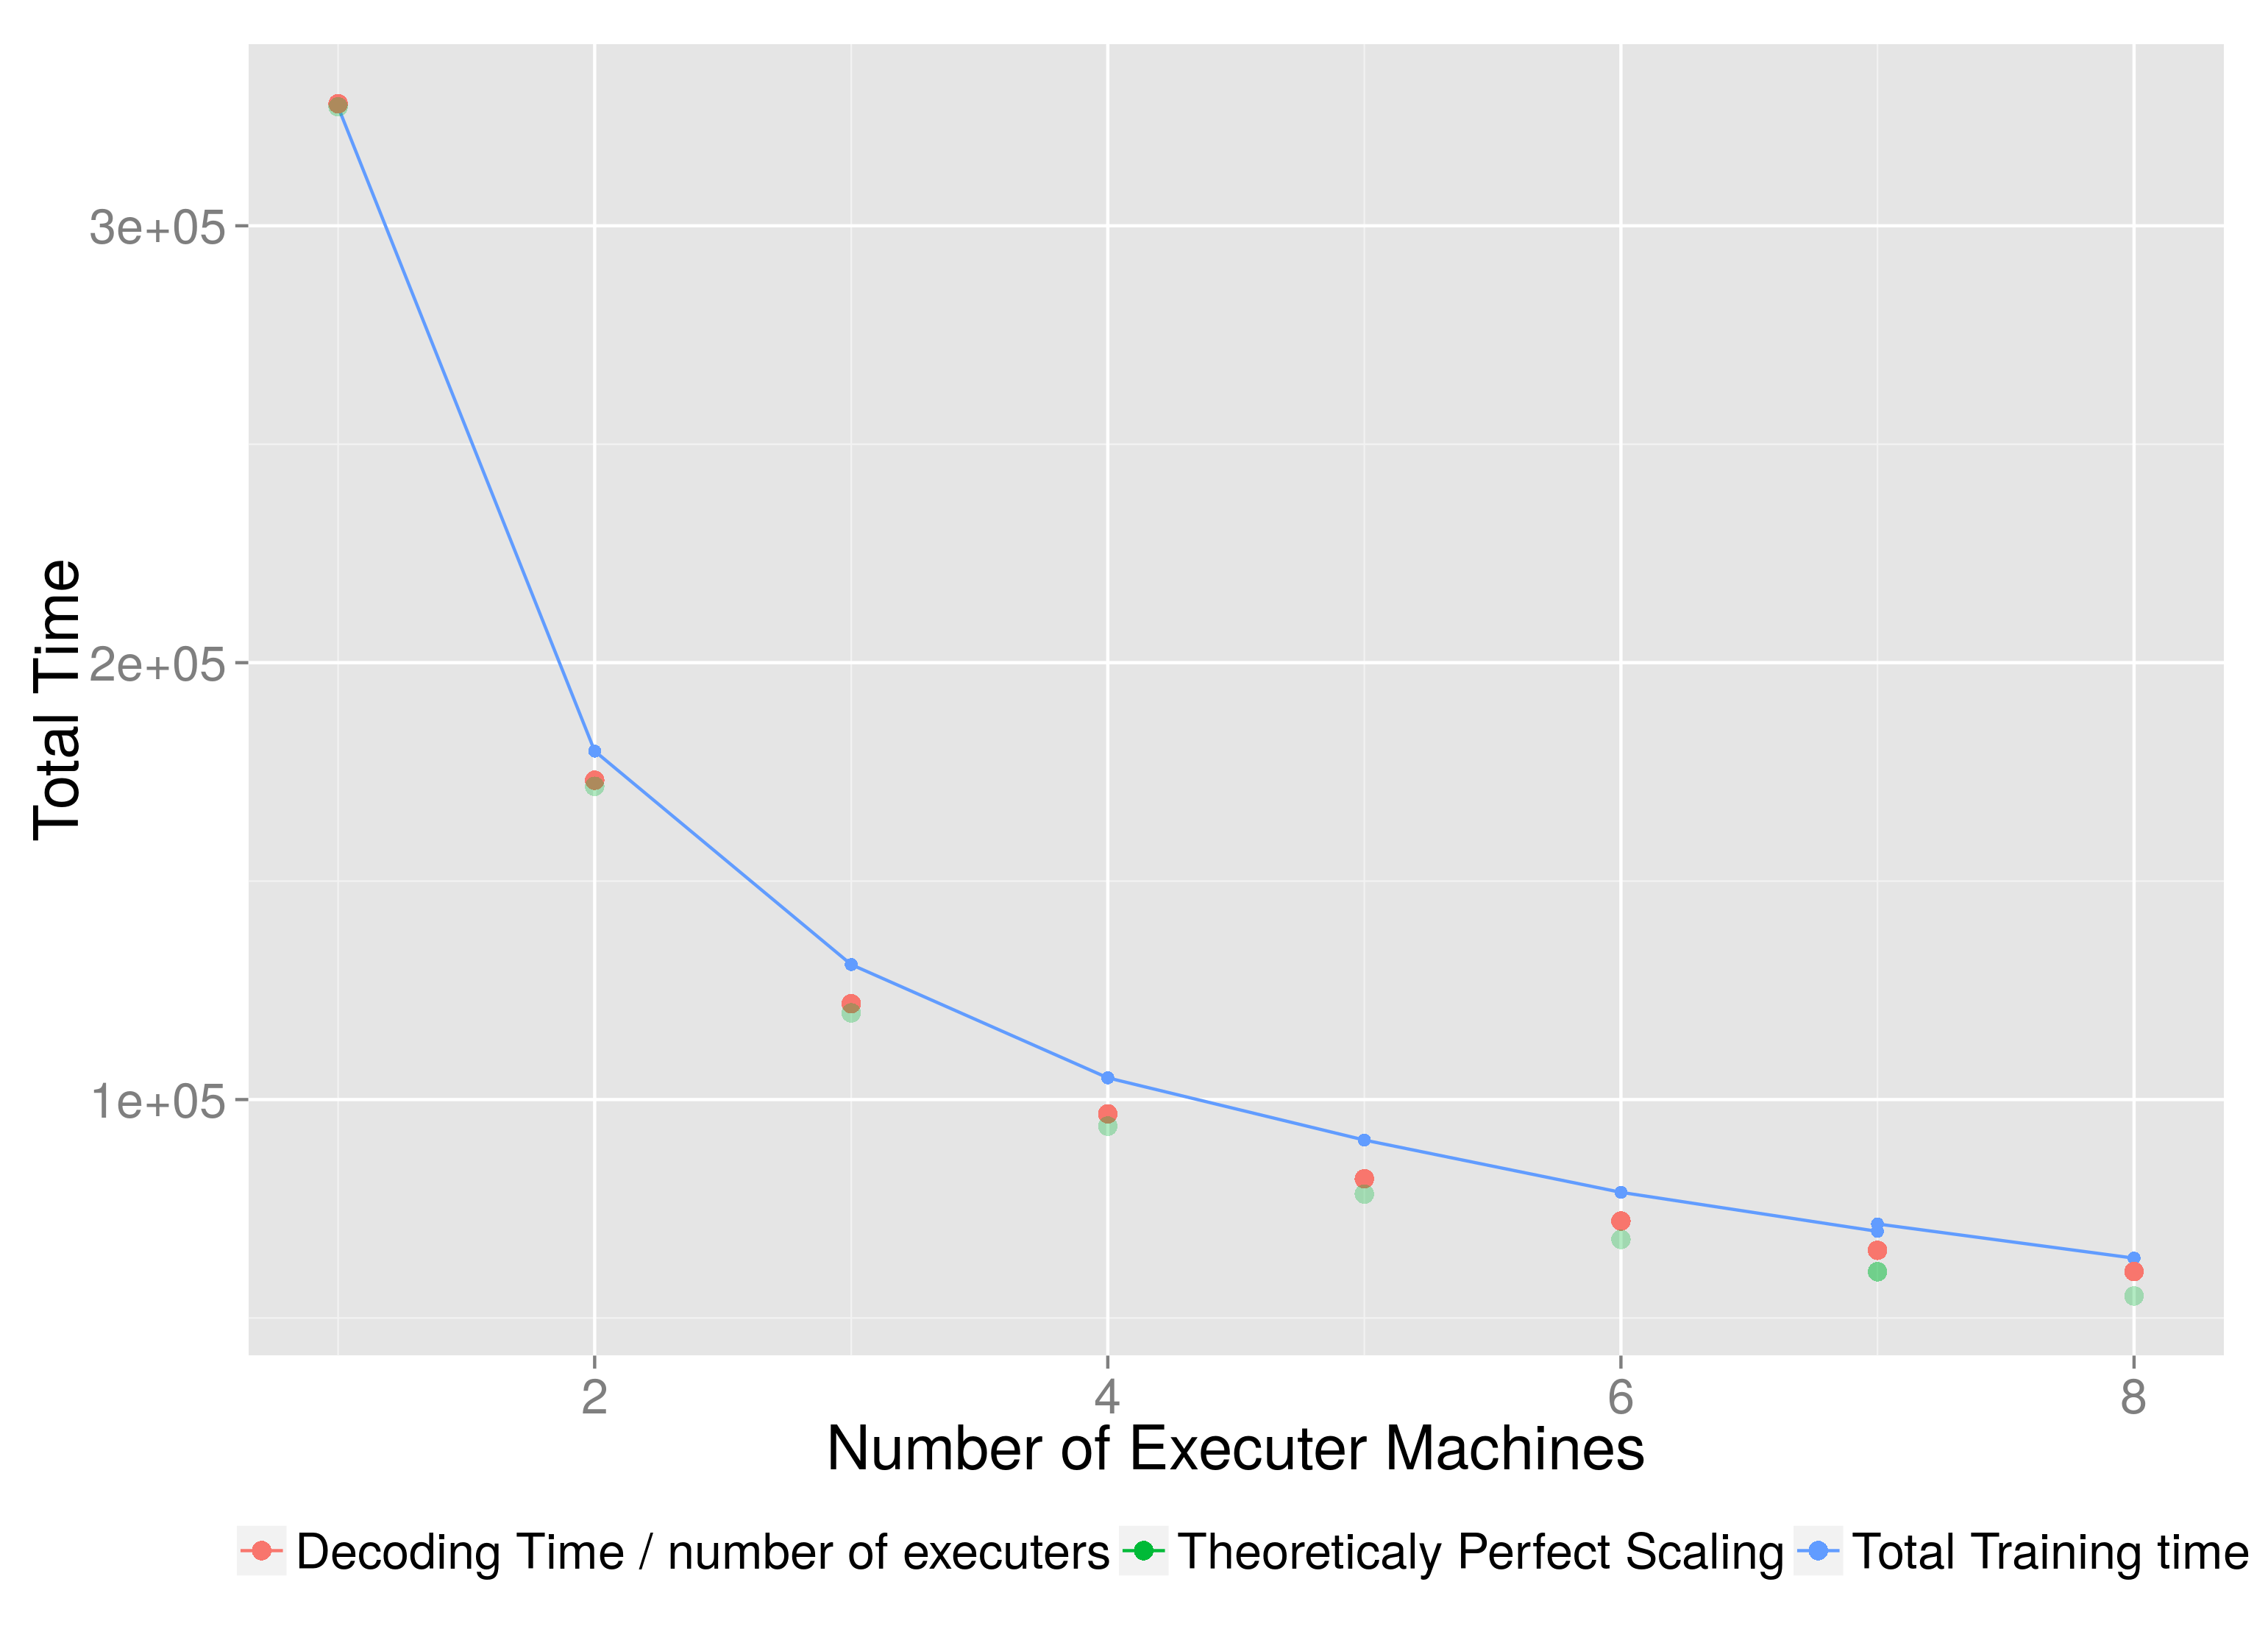
\includegraphics[width=1.0\textwidth]{images/scalabilityDistributed_msrc.png}
  \caption{ This Figure displays the total training time required for the entire MSRC data set on a varying number of m3.large AWS virtual machines each configured to use just one core. We can again see a good scaling curve as the true train time is close to the expected train time if there was no delay in context switching (Theoretically Perfect Scaling). Bu the scaling is not perfect and as more machines are added the difference in training time produced by additional time used on the driver node for recombination and coordination increases the distance to perfect scaling. } 
  \label{fig:scaleDistrmsrc1}
 
\end{figure}

